%     Mathematical analysis
%---------------------------------------------------------------------------------------------------
% file MA.tex
% Notes>
% Mezery v matematickém režimu:
%~~~~~~~~~~~~~~~~~~~~~~~~~~~~~~
%\! záporná uzká mezera,   \; široká mezera,   \ mezislovní mezera,
%\, úzká mezera,   \: střední mezera,   \quad čtverčík,   \qquad dva čtverčíky
%---------------------------------------------------------------------------------------------------
\lstset{ %
  language=Matlab,                       % choose the language of the code
  basicstyle=\footnotesize,              % the size of the fonts that are used for the code
  backgroundcolor=\color{White},         % choose the background color.
  commentstyle=\color{help}\textit,
  keywordstyle=\color{keyword}\textbf,
  breaklines=true,                       % sets automatic line breaking
  breakatwhitespace=true,                % sets if automatic breaks should only happen at whitespace
  showspaces=false,                      % show spaces adding particular underscores
  showstringspaces=true,                 % underline spaces within strings
  showtabs=true,                         % show tabs within strings adding particular underscores
  frame=none,	                           % adds a frame around the code - none, single
  tabsize=8,                             % sets default tabsize to 8 spaces
  captionpos=b,                          % sets the caption-position to bottom
  numbers=left,                          % where to put the line-numbers -none, left, right
  numberstyle=\footnotesize,             % the size of the fonts that are used for the line-numbers
  stepnumber=1,                          % the step between two line-numbers. If it's 1 each line
                                         % will be numbered
  xleftmargin=3em,                       % adjust left margin										 
}
%---------------------------------------------------------------------------------------------------
% Setting path to image 
\graphicspath{{../src/MAI/img/}}  
%--------------------Introduction to mathematical analysis -----------------------------------------
    % !TeX spellcheck = cs_CZ
%     An overview of high school mathematics

{\tikzset{external/prefix={tikz/MAI/}}
 \tikzset{external/figure name/.add={ch01_}{}}
%---------------------------------------------------------------------------------------------------
% intro_MA.tex
%---------------------------------------------------------------------------------------------------
\chapter{Historie matematické analýzy}\label{mai:IchapI}
\minitoc


  Analýza jako nezávislý předmět byla vytvořena v 17. stol. během vědecké revoluce. Kepler, 
  Galilei, Descartes, Fermat, Huygens, Newton a Leibniz, když zmíníme jen několik důležitých jmen 
  těch, kteří přispěli k jejímu vzniku. Otázky z mechaniky, optiky a astronomie hráli roli v jejím 
  raném období, tak jako vnitřní problémy matematiky, jako výpočet obsahů, objemů a analýza 
  komplikovaných křivek. Pohyb po zakřivených drahách působením proměnných sil, které se staly 
  předmětem důkladného zájmu po studiu volně padajících těles Galilea, vedl k počátečnímu úspěchu. 
  Z velké rozmanitosti snah, které se objevily na konci 17. stol. v práci Newtona a Leibnize, se 
  zrodila nová matematická disciplína, jejíž některé poznatky jsou v těchto studijních zápiscích.
  
  Základní myšlenka použití diferenciálních rovnic k získání pohledu na globální chování proměnných kvantit z jejich (infinitezimálních) změn prokázala základní a plodné výsledky daleko za hranicemi matematiky a fyzika a formovala náš souhrnný vědecký pohled na svět, zvláště na představu o kauzalitě. Na konci 18. stol., vskutku, největší vědci došli ke shodě, že procesy v přírodě (a společnosti) jsou determinovány a podřízeny zákonům, které mohou být popsány v podobě 
  diferenciálních rovnic. Laplace, tento mistr matematické fyziky, naznačil obraz nějaké fiktivní 
  vševědoucí inteligence, užívající úplnou znalost zákonů a stavu světa v daný časový okamžik, by 
  mohla předpovídat další vývoj světa navždy a hned. Myšlenka \emph{přírodních zákonů} byla kmotrem 
  při vytvoření matematického pojmu funkce a naopak nebyla by to myšlenka nikdy tak vlivná, kdyby 
  matematická analýza nevyvíjela úspěšné metody pro výzkum funkčních závislostí. 

} % tikzset
%---------------------------------------------------------------------------------------------------
%\printbibliography[title={Seznam literatury}, heading=subbibliography]
\addcontentsline{toc}{section}{Seznam literatury}
                
%---------------------Reálná a komplexní čísla------------------------------------------------------
    %----------------------------------------------------------------------------------------------------
% file Real_and_Complex_Numbers.tex
%----------------------------------------------------------------------------------------------------
\chapter{Reálná a komplexní čísla}
\minitoc
\newpage
%================Kapitola: Diferenciální rovnice 1. řádu ============================================

\printbibliography[title={Seznam literatury}, heading=subbibliography]
\addcontentsline{toc}{section}{Seznam literatury}     
%-------------------- Differential calculus --------------------------------------------------------
    %     Differential calculus
%--------------------------------------------------------------------------------------------------
% file Diff_calc.tex
%--------------------------------------------------------------------------------------------------
\chapter{Limita a spojitost funkce}\label{MA1:chap_Limita}
\minitoc
\newpage
  %================Podkapitola: Reálná funkce =====================================================
  \section{Reálná funkce}
    %----------------------------------------------------------------------------------------------
    \subsection{Pojem funkce}
    %----------------------------------------------------------------------------------------------
    \subsection{Graf funkce. Různé způsoby zadání funkce}
      Každé funkci můžeme přiřadit její graf. 
      \textbf{Grafem funkce} $f:A\rightarrow\realset,\ A\subset\realset$, rozumíme množinu všech bodů 
      euklidovské roviny, jejíž souřadnice $x$, $y$ v dané kartézské soustavě souřadnic vyhovuje rovnice 
      \begin{equation}\label{MAI:eq_graf04}
        y=f(x). 
      \end{equation}  
      
      Grafem funkce může v jednodušších případech posloužit jako prostředek k získání názorné       
      \textquotedblleft představy\textquotedblright. Grafy některých funkcí jsou \textquotedblleft 
      křivky\textquotedblright\, (intuitivním smyslu tohoto slova). Avšak u některých funkcí názorná 
      představa grafu selhává. Vezmeme-li např. Dirichletovu funkci z odst. **, snadno zjistíme, že její graf 
      nemůžeme sestrojit (byly by to \textquotedblleft dvě rovnoběžné přímky $y=0$ a $y=1$ s nekonečným 
      množstvím mezer\textquotedblright)
      
      Zadat funkci znamená udat její definiční obor a \textquotedblleft zobrazovací předpis 
      \textquotedblright, tj pravidlo (formulované slovně či v používaném matematickém jazyku), 
      podle něhož můžeme jednoznačným způsobem rozhodnout, jaká funkční hodnota odpovídá libovolně 
      zvolenému číslu z definičního oboru. Definičním oborem bývá často interval nebo sjednocení 
      intervalů. Není-li definiční obor udán, rozumíme jím množinu všech reálných čísel, pro něž je 
      příslušný předpis definován. Tuto množinu nazýváme \textbf{přirozeným (též maximálním) 
      definičním oborem funkce}. Je to tzv. \emph{existenční obor} výrazu, jímž je funkce definována 
      \cite[s.~84]{Brabec1989}.
      
      Například funkce $f: \realset\rightarrow\realset,\ f(x)=x^2$, můžeme vyjádřit bez udání definičního  
      oboru 
      $\realset$ vztahem 
      \begin{equation*}
        f: y=x^2,
      \end{equation*}
      neboť předpis $y=x^2$ má smysl pro každé reálné číslo $x$. Avšak u funkce 
      $g:\langle0,1\rangle\rightarrow\realset,\ g(x)=x^2,$ je nutné v zápisu funkce definiční obor 
      $\langle0,1\rangle$ uvést, píšeme tedy   
      \begin{equation*}
        g: y=x^2, \quad x\in\langle0,1\rangle.
      \end{equation*}
      Zobrazovací předpis, kterým je funkce zadána, může být rozmanitý. Nejčastěji a pro účely matematické 
      analýzy nejvhodnější je \emph{analytické zadání vzorcem}, tj. rovnicí tvaru $y=f(x)$ nebo několika 
      takovými rovnicemi platnými pro různé části definičního oboru. Přitom v rovnici $y=f(x)$ je na pravé 
      straně nějaký správně definovaný výraz obsahující nejvýše poměnnou $x$ a nabývající jednoznačné hodnoty 
      pro danou hodnotu proměnné $x$.

      \begin{example}\label{MAI:exam01} 
        Vzorcem $f(x)=\sqrt{1-x}$ je dána funkce, jejímž přirozeným oborem je interval $(-\infty,1\rangle$ 
        (uvažme, že výraz $\sqrt{1-x}$ je definován v reálném oboru, je-li $1-x\geq0$). Graf této funkce 
        je část paraboly, jejíš osou je osa $x$, viz obr. \ref{MAI:fig_diff_app_03}.
        %----------------------------------
        % image: MAI_diff_app_03.tex label: \label{MAI:fig_diff_app_03}
           % \documentclass{article}
% \usepackage{xltxtra} 
% \usepackage{tikz}
% \usetikzlibrary{decorations.markings}
% \usetikzlibrary{intersections}
% \usepackage{subfigure} 
% \usetikzlibrary{calc}
% 
% \newcommand{\MyXYcross}{%
%           \draw[name path=axeX,->] (\xmin,\zero) -- (\xmax,\zero)   node[right] {$x$} coordinate(x axis);
%           \draw[name path=axeY,->] (\phase,\ymin) -- (\phase,\ymax) node[left]  {$y$} coordinate(y axis);
%           \path[name intersections={of=axeX and axeY, name=pocatek}]; 
%           \node[below left] at (pocatek-1) {$0$};
%           \draw[fill=white] (pocatek-1) circle(2pt);  
% }
%\begin{document}

  \begin{figure}[htb]  
    \centering
        \def\xmin{-160}
        \def\xmax{100}
        \def\ymin{-15}
        \def\ymax{+100}
        \def\zero{0}
        \def\phase{0}
      \begin{tikzpicture}
        \begin{scope}[draw=black,line join=round, miter limit=4.00,line width=0.5pt,y=1pt,x=1pt] 
          \MyXYcross;   
        \end{scope}
        
        \begin{scope}[domain=-2:1, line join=round, miter limit=4.00,line width=0.5pt, 
                      x=50pt,y=50pt, xshift=0, yshift=0]    
         \draw[color=red] plot[id=myfce, samples=2000, smooth] function{sqrt(1-x)}; 
         % 
         \foreach \x/\xtext in {-1/1, -2/2, -3/3}
            \draw[shift={(\x,0)}] (0pt,2pt) -- (0pt,-2pt) node[below] {$\xtext$};
            
         \node at(2,1.2) [left, fill=white] {$f(x): y=\sqrt{1-x}$}; %   
         \draw[fill=black] (1,0) node[below] {$1$} circle(1pt);
          \draw[fill=black] (0,1) circle(1pt);  
          \node at (0,1) [left] {$1$};        
        \end{scope}  
      \end{tikzpicture}
    \caption{Graf funkce $y=\sqrt{1-x}$ je část paraboly, jejíž osou je osa $x$}\label{MAI:fig_diff_app_03}
  \end{figure}
  
%\end{document}  
        %----------------------------------         
      \end{example}   
      \begin{example}\label{MAI:exam07} 
        Funkce je dána vzorcem 
        \begin{equation*}
          f(x):y=\abs{x}.
        \end{equation*} 
        Přirozeným definičním oborem této funkce je množina $\realset$. Táž funkce může být dána i vzorcem
        \begin{equation*}
          f(x):y=\sqrt{x},
        \end{equation*}    
        nebo dvěma rovnicemi
        \begin{equation*}
          f(x):y=
             \begin{cases}
                 x & \text{je-li} x \geq 0. \\
                -x & \text{je-li} x < 0,
             \end{cases}                 
        \end{equation*}  
        což je zřejmé, uvědomíme-li si jak je definována absolutní hodnota. Graf funkce je na obr. 
        \ref{MAI:fig_diff_app_05}.
        %----------------------------------
        % image: MAI_diff_app_05.tex label: \label{MAI:fig_diff_app_05}
           % \documentclass{article}
% \usepackage{xltxtra} 
% \usepackage{tikz}
% \usetikzlibrary{decorations.markings}
% \usetikzlibrary{intersections}
% \usepackage{subfigure} 
% \usetikzlibrary{calc}
% \usepackage{amsmath, amsthm, amssymb, amsfonts, amsbsy}
% 
% \newcommand{\abs}[1]{\left\lvert#1\right\rvert} 
% \newcommand{\MyXYcross}{%
%           \draw[name path=axeX,->] (\xmin,\zero) -- (\xmax,\zero)   node[right] {$x$} coordinate(x axis);
%           \draw[name path=axeY,->] (\phase,\ymin) -- (\phase,\ymax) node[left]  {$y$} coordinate(y axis);
%           \path[name intersections={of=axeX and axeY, name=pocatek}]; 
%           \node[below left] at (pocatek-1) {$0$};
%           \draw[fill=white] (pocatek-1) circle(2pt);  
% }
% \begin{document}

  \begin{figure}[htb]  
    \centering
        \def\xmin{-100}
        \def\xmax{100}
        \def\ymin{-15}
        \def\ymax{+100}
        \def\zero{0}
        \def\phase{0}
      \begin{tikzpicture}
        \begin{scope}[draw=black,line join=round, miter limit=4.00,line width=0.5pt,y=1pt,x=1pt] 
          \MyXYcross;   
        \end{scope}
        
        \begin{scope}[domain=-1:1, line join=round, miter limit=4.00,line width=0.5pt, 
                      x=50pt,y=50pt, xshift=0, yshift=0]    
          \node at(2,1.2) [left, fill=white] {$f(x): y=\abs{x}$};   %                         
          \draw[color=red] plot[id=myfce, samples=2000, smooth] function{abs(x)}; % 
          
          \foreach \x/\xtext in {-1/1, 1/1}
            \draw[shift={(\x,0)}] (0pt,2pt) -- (0pt,-2pt) node[below] {$\xtext$};                 
        \end{scope}  
      \end{tikzpicture}
    \caption{Graf funkce $y=\abs{x}$}\label{MAI:fig_diff_app_05}
  \end{figure}
  
%\end{document}  
        %----------------------------------         
      \end{example}  
      Funkce může být analyticky zadána i jinak než vzorcem $y=f(x)$. časté je \textbf{parametrické 
      vyjadřování}, tj. vyjádření dvojicí rovnic 
      \begin{equation}\label{MAI:eq_graf02}
        x=\varphi(t),\ y=\psi(t),\ t\in J,
      \end{equation}
      kde $\varphi, \psi$ jsou funkce definované na množině $J$ ($\ J$ bývá obvykle interval). Proměnná $t$ 
      se nazývá \emph{parametr}: má zde pomocný význam. Zajímá nás totiž vztah mezi $x$ a $y$. Rovnice 
      \ref{MAI:eq_graf02} definuje relaci $f\subset\realset\times\realset=\realset^2$:
      \begin{equation}\label{MAI:eq_graf03}
        f = \{(x,y)\in\realset^2; \text{ existuje } t\in J \text{ tak, že } x=\varphi(t),\ y=\psi(t)\}.
      \end{equation}      
      Tato relace může být za určitých podmínek jednoznačná tj. je funkcí z $\realset$ do $\realset$. 
      V tomto případě říkáme, že funkce $f$ je \emph{definována parametricky rovnicemi \ref{MAI:eq_graf02}}
      
      \begin{example}\label{MAI:exam02}
        Rovnice $x=\cos t,\ y=\sin t\quad t\in\langle0,\pi\rangle$, definují parametricky funkci 
        \begin{equation}
          f: y= \sqrt{1-x^2}, \quad x\in\langle-1,1\rangle,
        \end{equation}
        jejíž grafem je polokružnice, ležící v horní polorovině $\{(x,y)\in\realset^2, y\geq0\}$.
        %----------------------------------
        % image: MAI_diff_app_04.tex label: \label{MAI_fig_diff_app_04}
           % \documentclass{article}
% \usepackage{xltxtra} 
% \usepackage{tikz}
% \usetikzlibrary{decorations.markings}
% \usetikzlibrary{intersections}
% \usepackage{subfigure} 
% \usetikzlibrary{calc}
% 
% \newcommand{\MyXYcross}{%
%           \draw[name path=axeX,->] (\xmin,\zero) -- (\xmax,\zero)   node[right] {$x$} coordinate(x axis);
%           \draw[name path=axeY,->] (\phase,\ymin) -- (\phase,\ymax) node[left]  {$y$} coordinate(y axis);
%           \path[name intersections={of=axeX and axeY, name=pocatek}]; 
%           \node[below left] at (pocatek-1) {$0$};
%           \draw[fill=white] (pocatek-1) circle(2pt);  
% }
% \begin{document}

  \begin{figure}[htb]  
    \centering
        \def\xmin{-100}
        \def\xmax{100}
        \def\ymin{-15}
        \def\ymax{+100}
        \def\zero{0}
        \def\phase{0}
      \begin{tikzpicture}
        \begin{scope}[draw=black,line join=round, miter limit=4.00,line width=0.5pt,y=1pt,x=1pt] 
          \MyXYcross;   
        \end{scope}
        
        \begin{scope}[domain=-1:1, line join=round, miter limit=4.00,line width=0.5pt, 
                      x=50pt,y=50pt, xshift=0, yshift=0]    
          \node at(2,1.2) [left, fill=white] {$f(x): y=\sqrt{1-x}$};    %                         
          \draw[color=red] plot[id=myfce, samples=200, smooth] function{sqrt(1-x*x)}; %    
          \draw[fill=black] (+1,0) node[below] {$1$}  circle(1pt);
          \draw[fill=black] (-1,0) node[below] {$-1$} circle(1pt);
          \draw[fill=black] (0,1) circle(1pt);  
          \node at (0,1) [left] {$1$};        
        \end{scope}  
      \end{tikzpicture}
    \caption{Graf funkce $y=\sqrt{1-x}$ je polokružnice}\label{MAI:fig_diff_app_04}
  \end{figure}
  
%\end{document}  
        %----------------------------------         
      \end{example}
      Blíže se parametrickým zadáním funkce budeme zabívat v kapitole \ref{chap:Apl_dif_poc} (Aplikace 
      diferenciálního počtu).
      
      Funkce může být někdy zadána též rovnicí tvaru 
      \begin{equation}\label{MAI:eq_graf01}
        F(x,y) = 0.
      \end{equation}
      Přitom $F$ je funkce dvou proměnných, tj. zobrazení z $\realset^2\rightarrow\realset$. Kromě rovnice 
      \ref{MAI:eq_graf01} může být dána ještě podmínka, aby bod $(x,y)$ patřil k některé množině 
      $M\subset\realset^2$. Rovnicí \ref{MAI:eq_graf01} je definován opět jakási relace 
      $f\subset\realset\times\realset$,
      \begin{equation}
        f = \{(x,y)\in\realset^2,\quad F(x,y)=0 \}
      \end{equation}
      (případně $f = \{(x,y)\in\realset^2,\ F(x,y)=0,\ (x,y)\in M \}$), zajímá nás, kdy tato relace je 
      funkcí z $\realset$ do $\realset$. Říkáme pak, že funke $f$ je dána \textbf{implicitně} uvedenou 
      rovnicí \ref{MAI:eq_graf01} (příp. rovnicí \ref{MAI:eq_graf01} a podmínkou $(x,y)\in M$). 
      Naproti tomu zadání funkce ve tvaru 
      $y=f(x)$ nazýváme \textbf{explicitním}.
      
      \begin{example}\label{MAI:exam03} 
        Rovnicí $x+2y-3=0$ je implicitně definována funkce $f:y=-\dfrac{1}{2}x+\dfrac{3}{2}$.
      \end{example}
      \begin{example}\label{MAI:exam04} 
        Rovnicí $x^2+y^2=1$ a podmínkou $y\geq0$ je definována implicitní funkce z příkladu \ref{MAI:exam02}. 
        Relace $\{(x,y)\in\realset^2;\ x^2+y^2=1\}$ není ovšem jednoznačná, každé hodnotě $x\in(-1,1)$ 
        odpovídají dvě hodnoty $y: y_1=\sqrt{1-x^2}$, $y: y_2=-\sqrt{1-x^2}$. Podmínkou $y\geq0$ druhou 
        hodnotu vylučujeme. Místo podmínky $y\geq0$ bychom mohli uvést i jiné podmínky, aby rovnice 
        $x^2+y^2=1$ určovala implicitní funkci.   
      \end{example}
      
      Vyšetřování podminek, při nichž rovnice $F(x,y)=0$ je definována funkce $f$, se obvykle provádí 
      metodami matematické analýzy funkce více proměnných. 
      
      Funkce může být někdy dána tabulkou, tj. dvojicemi hodnot argumentu a funkce, což bývá obvyklé při 
      zjišťování závislosti veličin měřením. Proměnná $x$ se v tomto případě mění \textquotedblleft 
      diskrétně\textquotedblright. Je zřejmé, že tímto způsobem můžeme definovat úplně jen tehdy, je-li 
      definiční obor konečná množina. Tabulku však používáme i v jiných případech, zejména chceme-li vyznačit 
      pomocí ní, některé hodnoty, 
      které nás z nějakého důvodu přednostně zajímají. 
      
      V technických aplikacích bývá funkce dána graficky. Z grafu můžeme ovšem funkční hodnoty určit pouze 
      přibližně. Pro další matematické zpracování je grafické zadání nejméně vhodné, i když jeho praktický 
      význam nelze popřít. 
      
      Speciálním případem reálných funkcí jedné realné proměnné jsou \emph{posloupnosti reálných čísel}. 
         
    %----------------------------------------------------------------------------------------------        
    \subsection{Některé zvláštní vlastnosti funkcí}\label{MA1:subsec_vlastnosti_funkce}
      \subsubsection{Omezená funkce}
        \begin{definition}\label{MA1:def_lim01}
          Funkci $f$ nazýváme shora (zdola) omezenou na množině $A\subset D(f)$, je-li shora (zdola) omezená 
          množina funkčních hodnot $f(A)$. Je-li funkce $f$ omezená shora i zdola na množině $A$, pak ji 
          nazýváme omezenou na množině $A$. Je-li $A=D(f)$, nazýváme funkci omezenou. Viz kniha 
          \cite[s.~87]{Brabec1989}       
        \end{definition}
        Funkce $f$ je omezená na množině $A$, právě když existuje číslo $K>0$ tak, že platí
        $$|f(x)|\leq K \qquad \text{pro každé } x\in A$$
        neboli
        $$-K\leq f(x) \leq K \qquad \text{pro každé } x\in A.$$
        \begin{example}\label{MAI:exam05}
          Funkce $f:y=\frac{1}{x^2+1}$ je omezená. Platí totiž $$\left|\frac{1}{x^2+1}\right|=\frac{1}{x^2+1}\leq1 \qquad \text{pro všechna }x\in\realset.$$ Zdola
          je tato funkce omezena dokonce číslem $0$.  
        \end{example}
        \begin{itemize}
          \item Je-li funkce $f$ shora omezená na množině $A$, existuje konečné \emph{supremum} $\sup f(A)$. 
                Toto číslo nazýváme \emph{supremem funkce $f$ na množině $A$} a označujeme je též $\sup_{x\in 
                A}f(A)$ nebo $\sup\{f(x), x\in A\}$.
          \item Je-li funkce $f$ zdola omezená na množině $A$, existuje konečné \emph{infimum} $\inf(A)$,    
                které nazýváme \emph{infimum funkce $f$ na množině $A$} a označujeme je též $\inf_{x\in 
                A}f(A)$ nebo $\inf\{f(x), x\in A\}$. 
          \item Není-li funcke $f$ shoda (zdola) omezená na množině $A$, pak je ovšem $\sup_{x\in A}    
                f(x)=+\infty$ ($\sup_{x\in A} f(x)=-\infty$).
          \item Má-li množina $f(A)$ největší (nejmenší) prvek, pak toto číslo nazýváme největší 
                (nejmenší hodnotou funkce $f$  na množině $A$ (je-li $A = f(f)$, též absolutním maximem, 
                resp. absolutním minimem funkce $f$) a značíme je $\max_{x\in A} f(x)$ ($\min_{x\in A} 
                f(x)$). V tomto případě existuje takové číslo $x_0\in A$, že $f(x_0)=\max_{x\in A}f(x)$ 
                ($f(x_0)=\min_{x\in A}f(x)$). Pro všechna $x\in A$ tedy platí $f(x)\leq f(x_0)$ 
                ($f(x)\geq f(x_0)$). Je zřejmé, že největší (nejmenší) hodnota funkce $f$ na množině $A$, 
                pokud existuje je současně supremem (infimem) funkce $f$ na $A$.
        \end{itemize}
        \begin{example}\label{MAI:exam06}
          Pro funkci z příkladu \ref{MAI:exam05} platí:
          \begin{equation}
            \sup_{x\in\realset}=\frac{1}{x^2+1}=\max_{x\in\realset}=\frac{1}{x^2+1}=1; \qquad \inf_{x\in\realset}=\frac{1}{x^2+1}=0,
          \end{equation}
          tato funkce však nenabývá v definičním oboru $\realset$ nejmenší hodnoty, neboť je stále 
          $\dfrac{1}{x^2+1}>0$. To, že infimum je $0$, dokážeme takto: Zvolíme-li libovolně $\varepsilon>0$, 
          pak snadno zjistíme, že existuje $x$, pro níž $\dfrac{1}{x^2+1}<\varepsilon$:
          \begin{align*}
            1                  &< \varepsilon(x^2+1) \\
            \frac{1}{\epsilon} &< x^2+1 \Rightarrow \sqrt{\frac{1}{\epsilon}-1} < x
          \end{align*} 
          %----------------------------------
          % image: MAI_rolle_01.tex label: \label{MAI:fig_diff_app_02}
            % \documentclass{article}
% \usepackage{tikz}
% \usetikzlibrary{decorations.markings}
% \usetikzlibrary{intersections}
% \usepackage{subfigure} 
% \usetikzlibrary{calc}
% 
% \newcommand{\MyXYcross}{%
%    \draw[name path=axeX,->] (\xmin,\zero) -- (\xmax,\zero)   node[right] {$x$} coordinate(x axis);
%    \draw[name path=axeY,->] (\phase,\ymin) -- (\phase,\ymax) node[left]  {$y$} coordinate(y axis);
%    \path[name intersections={of=axeX and axeY, name=pocatek}]; 
%    \node[below left] at (pocatek-1) {$0$};
%    \draw[fill=white] (pocatek-1) circle(2pt);  
% }
%  \begin{document}
 
  \begin{figure}[htb]  
    \centering
        \def\xmin{-150}
        \def\xmax{150}
        \def\ymin{-15}
        \def\ymax{+90}
        \def\zero{0}
        \def\phase{0}
	  \begin{tikzpicture}
		\begin{scope}[draw=black,line join=round, miter limit=4.00,line width=0.5pt,y=1pt,x=1pt] 
          \MyXYcross;	
        \end{scope}
		
        \begin{scope}[domain=-2.5:2.5, line join=round, miter limit=4.00,line width=0.5pt, 
		              x=50pt,y=50pt, xshift=0, yshift=0]		
		  \draw[name path=fce, color=blue, smooth]   
		      plot[mark=triangle*] (\x,{1/(\x*\x+1)}); % 
		  \node at(2.5,1) [left, fill=white] {$f(x):y=\frac{1}{1+x^2}$};	
          \draw[dashed] (0,0.5) node[left] {$\frac{1}{2}$} -- ++(1,0) -- ++(0,-0.5) node[below] {$1$} ;
          \draw[fill=black] (1,0.5) circle(1pt);
          \draw[fill=black] (0,1) circle(1pt);	
          \node at (0,1) [left] {$1$};		  
		\end{scope}  
	  \end{tikzpicture}
    \caption{ }\label{MAI:fig_diff_app_02}
  \end{figure}
  
% \end{document}  
          %----------------------------------           
          Neexistuje tedy kladné číslo, jíž by bylo dolní mezí množiny funkčních hodnot, takže infimum je $0$. Graf funkce $f$ je na obr. \ref{MAI:fig_diff_app_02}.
        \end{example}
       
      \subsubsection{Monotonní funkce}
        \begin{definition}\label{MA1:def_lim02}
          Funkci $f$ nazýváme \textbf{rostoucí (klesající)} na množině $A\subset D(f)$, jestliže pro každé 
          dva body $x_1, x_2\in A,\ x_1<x_2$, platí $f(x_1)<f(x_2)$ ($f(x_1)>f(x_2)$). Funkci $f$ nazýváme 
          \textbf{neklesající (nerostoucí)} na množině $A\subset D(f)$, jestliže pro každé dvá body $x_1, 
          x_2\in A,x_1<x_2$, platí $f(x_1)\leq f(x_2)$ ($f(x_1)\geq f(x_2)$). Rostoucí a klesající funkce (na 
          množině $A$) se nazývají \textbf{ryze monotónní} (na množině $A$), neklesající a nerostoucí funkce 
          (na množině $A$) se nazývají monotónní (na množině $A$).    
        \end{definition}
            
        Z definice je zřejmé, že každá rostoucí funkce je zároveň neklesající a každá klesající funkce je 
        zároveň nerostoucí. Ryze monotónní funkce tvoří tedy podmnožinu množiny monotónních funkcí. 
           
        \begin{example}
          Funkce $y=2x+1$ je \textbf{rostoucí} na intervalu $(-\infty, \infty)$. Platí totiž: $x_1<x_2\Rightarrow 2x_1<2x_2\Rightarrow2x_1+1<2x_2+1$.
        \end{example}
        \begin{example}
          Funkce y=[x] je \textbf{neklesající} na intervalu $(-\infty, \infty)$ (viz příklad **). 
        \end{example}
        \begin{example}
          Heavisideova funkce (viz příklad **) je \textbf{neklesající} na intervalu $(-\infty, \infty)$ (viz příklad **). 
        \end{example}       
        \begin{example}
          Funkce $y=|x|$ je \textbf{klesající} na intervalu $(-\infty, 0\rangle$ a rostoucí na intervalu $\langle0, \infty)$. 
        \end{example}  
            
        \begin{definition}\label{MA1:def_lim03}
          Funkci $f$ nazýváme \textbf{konstantí} na množině $A$, jestliže pro každé dva body $x_1, x_2\in A$, platí $f(x_1)=f(x_2)$. V tom případě existuje reálné číslo $k$ 
          takové, že pro každé $x\in A$ je $f(x)=k$. Je-li $k=0$, mluvíme o nulové funkci na množině $A$. 
        \end{definition} 
          
        Výrok ``funkce $f$ je konstantní na množině $A$'' zapisujeme též $f(x)=\text{konst na }A$. Funkci konstantní na $\realset$ budeme stručně nazývat \textbf{konstantní funkcí}
        nebo krátce \textbf{konstantou}. Z textu bude obvykle patrno, interpretujeme-li symbol $k$ jako reálné číslo nebo jako konstantní funkci. Je zřejmé, že konstantní funkce
        na množině $A$ je zároveň neklesající i nerostoucí na množině $A$. Toto tvrzení se dá obrátit. Lze snadno dokázat i tuto větu:        
        \begin{lemma}\label{MA1:lem_lim01}
          Funkce $f$ je \textbf{rostoucí} na množině $A$, právě když je neklesající na množině $A$ a na žádné dvoubodové podmnožině $B\subset A$ není konstantní. 
        \end{lemma}
        Obdobná tvrzení platí i pro klesající funkce. 
               
      \subsubsection{Sudé a liché funkce}
        \begin{definition}\label{MA1:def_lim04}
          Funkce $f$ se nazývá \textbf{sudá} jestliže pro každé $x\in D(f)$ je též $-x\in D(f)$
          a platí $f(x)=f(-x)$.
          Funkce $f$ se nazývá \textbf{lichá} jestliže pro každé $x\in D(f)$ je též $-x\in D(f)$
          a platí $f(-x)=-f(x)$. 
        \end{definition}
        Graf sudé funkce je souměrný podle osy $y$ (osy funkčních hodnot), graf liché funkce je 
        souměrný podle počátku. 
        \begin{example}\label{MAI:exam08}
          Funkce $f:\,y=x^2$ je sudá, funkce $g:\,y=x^3$ je lichá.
          %----------------------------------
          % image: MAI_diff_app_06.tex label: \label{MAI:fig_diff_app_06}
            % \documentclass{article}
% \usepackage{xltxtra} 
% \usepackage{tikz}
% \usetikzlibrary{decorations.markings}
% \usetikzlibrary{intersections}
% \usepackage{subfig} 
% \usetikzlibrary{calc}
% \usepackage{amsmath, amsthm, amssymb, amsfonts, amsbsy}
% 
% \newcommand{\abs}[1]{\left\lvert#1\right\rvert} 
% \newcommand{\MyXYcross}{%
%           \draw[name path=axeX,->] (\xmin,\zero) -- (\xmax,\zero)   node[right] {$x$} coordinate(x axis);
%           \draw[name path=axeY,->] (\phase,\ymin) -- (\phase,\ymax) node[left]  {$y$} coordinate(y axis);
%           \path[name intersections={of=axeX and axeY, name=pocatek}]; 
%           \node[below left] at (pocatek-1) {$0$};
%           \draw[fill=white] (pocatek-1) circle(2pt);  
% }
% \begin{document}

  \begin{figure}[htb]  
    \centering
        \def\xmin{-80}
        \def\xmax{80}
        \def\ymin{-100}
        \def\ymax{+120}
        \def\zero{0}
        \def\phase{0}
    \subfloat[sudá funkce]{     
      \begin{tikzpicture}
        \begin{scope}[draw=black,line join=round, miter limit=4.00,line width=0.5pt,y=1pt,x=1pt] 
          \MyXYcross;   
        \end{scope}
        
        \begin{scope}[domain=-1.2:1.2, line join=round, miter limit=4.00,line width=0.5pt, 
                      x=50pt,y=50pt, xshift=0, yshift=0]    
          \node at(1.9,1.6) [left, fill=white] {$f(x): y=x^2$}; %                         
          \draw[color=red] plot[id=myfce, samples=2000, smooth] function{x*x}; %          
          \foreach \x/\xtext in {-1/1, 1/1}
            \draw[shift={(\x,0)}] (0pt,2pt) -- (0pt,-2pt) node[below] {$\xtext$};                 
        \end{scope}  
      \end{tikzpicture}
    }
    \subfloat[lichá funkce]{    
      \begin{tikzpicture}
        \begin{scope}[draw=black,line join=round, miter limit=4.00,line width=0.5pt,y=1pt,x=1pt] 
          \MyXYcross;   
        \end{scope}
        
        \begin{scope}[domain=-1.2:1.2, line join=round, miter limit=4.00,line width=0.5pt, 
                      x=50pt,y=50pt, xshift=0, yshift=0]    
          \node at(1.8,1.9) [left, fill=white] {$g(x): y=x^3$}; %                         
          \draw[color=red] plot[id=myfce, samples=2000, smooth] function{x*x*x}; %        
          \foreach \x/\xtext in {-1/1, 1/1}
            \draw[shift={(\x,0)}] (0pt,2pt) -- (0pt,-2pt) node[below] {$\xtext$};                 
        \end{scope}  
      \end{tikzpicture}
    }   
    \caption{Příklad sudé a liché funkce}\label{MAI:fig_diff_app_06}
  \end{figure}
  
%\end{document}  
          %----------------------------------           
        \end{example}
        Daná funkce nemusí být ovšem ani sudá, ani lichá. Snadno se dokáže tvrzení:
        \begin{itemize}
          \item Je-li sudá funkce $f$ na množině $D(f)\cap\langle0,\infty)$ rostoucí (klesající),
                je na množině $D(f)\cap(-\infty,0\rangle$ klesající (rostoucí).
          \item Je-li lichá funkce na množině $D(f)\cap\langle0,\infty)$ rostoucí (klesající),
                je též na množině $D(f)\cap(-\infty,0\rangle$ klesající (rostoucí).                 
        \end{itemize}
      \subsubsection{Periodická funkce}
    %----------------------------------------------------------------------------------------------      
    \subsection{Operace s funkcemi. Uspořádání}       
    
    %----------------------------------------------------------------------------------------------
    \subsection{Elementární funkce}
      Základními elementárními funkcemi nazýváme \cite[s.~10]{PolakMA1}:
      \begin{displaymath}
        \xymatrix{
        \mbox{mocninné} & *+[F]{\mbox{Elementární funkce}}\ar@{->}[l]\ar@{->}[dl]\ar@{->}[d]\ar@{->}[dr]\ar@{->}[r]& \mbox{exponenciální}   \\
        \mbox{goniometrické}       &   \mbox{logaritmické}      & \mbox{cyklometrické}
        }
      \end{displaymath}
  
      \subsubsection{Goniometrické funkce}
      
        \begin{itemize}
          \item \textbf{Základní vzorce pro goniometrické funkce}
            \begin{align}
              \sin^2\alpha &+ \cos^2\alpha = 1      &\forall\alpha\in\realset \label{MA1:eq_sincos} \\ 
              |\sin\alpha| &= \sqrt{1-\cos^2\alpha} &\forall\alpha\in\realset \label{MA1:eq_sinabs} \\ 
              |\cos\alpha| &= \sqrt{1-\sin^2\alpha} &\forall\alpha\in\realset \label{MA1:eq_cosabs}
            \end{align}  
          \item \textbf{Součtové vzorce}
            \begin{align}
            % \nonumber to remove numbering (before each equation)
              \sin(\alpha + \beta) 
                &= \sin\alpha\cdot\cos\beta - \sin\beta\cdot\cos\alpha           \label{MA1:eq_sinxpy}  \\ 
              \sin(\alpha - \beta) 
                &= \sin\alpha\cdot\cos\beta + \sin\beta\cdot\cos\alpha           \label{MA1:eq_sinxmy}  \\ 
              \cos(\alpha + \beta) 
                &= \cos\alpha\cdot\cos\beta - \sin\alpha\cdot\sin\beta           \label{MA1:eq_cosxpy}  \\ 
              \cos(\alpha - \beta) 
                &= \cos\alpha\cdot\cos\beta + \sin\alpha\cdot\sin\beta           \label{MA1:eq_cosxmy}  \\ 
              \tan(\alpha\pm\beta) 
                &= \frac{\tan\alpha\pm\tan\beta}{1\mp\tan\alpha\cdot\tan\beta}   \label{MA1:eq_tanxpmy} \\ 
              \cot(\alpha\pm\beta) 
                &= \frac{1\mp\cot\alpha\cdot\cot\beta}{\cot\alpha\pm \cot\beta}  \label{MA1:eq_cotxpmy}
            \end{align}
            Součtové vzorce lze odvodit několika způsoby; jednoduchý způsob důkazu lze provést pomocí skalárního součinu vektorů.
          \item \textbf{Vzorce pro dvojnásobný úhel $2\alpha$}
            \newline Pro každé $\alpha\in R$ platí:
            \begin{align}
              \sin(2\alpha)   &= 2\sin\alpha\cos\alpha                \label{MA1:eq_sin2x} \\ 
              \cos(2\alpha)   &= \cos^2\alpha - \sin^2\alpha          \label{MA1:eq_cos2x} \\ 
              \tan(2\alpha)   &= \frac{2\tan\alpha}{1-\tan^2\alpha}   \label{MA1:eq_tan2x} \\ 
              \cot(2\alpha)   &= \frac{\cot^2\alpha - 1}{2\cot\alpha}                               \label{MA1:eq_cot2x}
            \end{align}
          \item \textbf{Vzorce pro poloviční úhel $\displaystyle\frac{\alpha}{2}$}
            \begin{align}
              \left|\sin\frac{\alpha}{2}\right|   
                &= \sqrt{\frac{1-\cos\alpha}{2}}                      \label{MA1:eq_sinx2} \\ 
              \left|\cos\frac{\alpha}{2}\right|   
                &= \sqrt{\frac{1+\cos\alpha}{2}}                      \label{MA1:eq_cosx2} \\ 
              \left|\tan\frac{\alpha}{2}\right|   
                &= \sqrt{\frac{1-\cos\alpha}{1+\cos\alpha}}           \label{MA1:eq_tanx2} \\ 
              \left|\cot\frac{\alpha}{2}\right|   
                &= \sqrt{\frac{1+\cos\alpha}{1-\cos\alpha}}           \label{MA1:eq_cotx2}
            \end{align}
        \end{itemize}
        Vzorce \ref{MA1:eq_sinx2} a \ref{MA1:eq_cosx2} odvodíme pomocí vzorců \ref{MA1:eq_cos2x} a \ref{MA1:eq_sincos}:
        \begin{align*}
          \cos\alpha &= 
          \cos2\frac{\alpha}{2}=\cos^2\frac{\alpha}{2}-\sin^2\frac{\alpha}{2}=1-2\sin^2\frac{\alpha}{2} \\
          \sin^2\frac{\alpha}{2} &= \frac{1-\cos\alpha}{2}   \\
          \cos^2\frac{\alpha}{2} &= 1 - \sin^2\frac{\alpha}{2} = \frac{1+\cos\alpha}{2} 
        \end{align*}
        a dále užijeme vztahu $\sqrt{a^2}=|a|$ (platí pro každé $a\in\realset$). Užitím součtových vzorců a 
        toho že, $\sin\frac{\pi}{2} = 1$, $\cos\frac{\pi}{2} = 0$, $\sin\pi = 0$ a $\cos\pi = -1$ lze snadno 
        odvodit, že pro každé 
        $\alpha\in R$ platí

        \begin{align*}
          \sin\left(\frac{\pi}{2}+\alpha\right) &=  \cos\alpha  &   \cos\left(\frac{\pi}{2}+\alpha\right) &= -\sin\alpha \\
          \sin\left(\frac{\pi}{2}-\alpha\right) &=  \cos\alpha  &   \cos\left(\frac{\pi}{2}-\alpha\right) &=  \sin\alpha \\
          \sin\left(\pi+\alpha\right)           &= -\sin\alpha  &   \cos\left(\pi+\alpha\right)           &= -\cos\alpha \\
          \sin\left(\pi-\alpha\right)           &=  \sin\alpha  &   \cos\left(\pi-\alpha\right)           &= -\cos\alpha \\
        \end{align*}
        \newline Důkaz provedeme pro první z těchto často užitečných vzorců (u ostatních je odvození obdobné):
        $$\sin\left(\frac{\pi}{2}+\alpha\right) = \sin\frac{\pi}{2}\cos\alpha + \cos\frac{\pi}{2}\sin\alpha = 1\cdot\cos\alpha + 0\cdot\sin\alpha.$$

    %---------------------------------------------------------------------------------------------- 
    \subsection{Zobrazení v jiných strukturách}
    
    %---------------------------------------------------------------------------------------------- 
    \subsection{Cvičení}
  %================Podkapitola: Limita funkce =============================================          
  \section{Limita funkce}
  
  %================Podkapitola: Spojitost funkce ==========================================        
  \section{Spojitost funkce}
  
%~~~~~~~~~~~~~~~~~~~~~~~~~~~~~~~~~~~~~~~~~~~~~~~~~~~~~~~~~~~~~~~~~~~~~~~~~~~~~~~~~~~~~~~~~~~~~~~~~~        
\printbibliography[title={Seznam literatury}, heading=subbibliography]
\addcontentsline{toc}{section}{Seznam literatury}          	 
%-------------------- Theory_of_Derivatives --------------------------------------------------------
    %----------------------------------------------------------------------------------------------------
% file: Theory_of_Derivates.tex
%----------------------------------------------------------------------------------------------------
\chapter{Derivace funkce}
\minitoc
\newpage
%================Kapitola: Derivace funkce ==========================================================
  \section{Základní věty diferenciálního počtu}
    \subsection{Věta o největší (nejmenší) hodnotě funkce}
      V tomto článku uvedeme významné věty, zvané souhrně věty o \emph{střední hodnotě diferenciálního počtu}, a dále pak ukázky jejich užití v matematické analýze. 
      Avšak dříve než budeme tyto věty formulovat, uvedeme jedno důležité tvrzení, které sice bude mít v dalších úvahách tohoto článku pomocnou úlohu, ale v teorii 
      extrémů má i samostatný význam. \cite[s.~186]{Brabec1989} 
      \begin{lemma}\label{MA1:lem_diff02}
        Nechť funkce $f:A\rightarrow\realset$ nabývá na množině $A$ své největší (nejmenší) hodnoty na vnitřním bodě $c$ množiny $A$. Máli funkce $f$ v bodě $c$ 
        derivaci, potom $f'(c)=0$.  
      \end{lemma}
      \begin{proof}
        Nechť např. $f(c)$ je největší hodnota funkce $f$ na množině $A$, takže $f(x)\leq f(c)$ pro $\forall x\in A$. Potom pro $x\in A, x<c$, je 
        $$\frac{f(x)-f(c)}{x-c}\geq 0$$
        a tedy
        $$f'_{-}(c)=\lim_{x\rightarrow c^-}\frac{f(x)-f(c)}{x-c}\geq0$$ 
        Dále pro $x\in A, x>c$, je
        $$\frac{f(x)-f(c)}{x-c}\leq 0$$ 
        a proto
        $$f'_{+}(c)=\lim_{x\rightarrow c^+}\frac{f(x)-f(c)}{x-c}\leq0$$
        Platí tedy
        $$f'_{+}(c)\leq f'_{-}(c)\geq f'_{-}(c).$$ 
        Avšak $f'_{+}(c)=f'_{-}(c)= f'(c)$. Odtud plyne $f'(c)=0$. 
      \end{proof}
      
    \subsection{Věty o střední hodnotě}
      \begin{lemma}\label{MA1:lem_diff03}
        \textbf{Rolleova věta}\footnote{Michel Rolle [Mišel Rol] (1652-1719) Francouzský matematik} Nechť funkce $f$ má tyto vlastnosti:
          \begin{enumerate}
            \item je spojitá na uzavřeném intervalu $\langle a,b\rangle$;
            \item má derivaci (vlastní či nevlastní) na otevřeném intervalu $(a,b)$;
            \item platí $f(a)=f(b)$.
          \end{enumerate}
        Potom v otevřeném intervalu $(a,b)$ existuje aspoň jeden bod $\xi$ takový, že $f'(\xi)=0$.   
      \end{lemma}
      \begin{proof}
        Protože je funkce $f$ je na uzavřeném intervalu $\langle a,b\rangle$ spojitá, nabývá v tomto intervalu své největší hodnoty $M$,
        své nejmenší hodnoty $m$. Přitom ovšem platí:
        \begin{equation}\label{MA1:eq_diff02}
          m\leq f(x) \leq M, \qquad x\in\langle a,b\rangle.
        \end{equation}
        Nyní mohou nastat dva případy: 
        \begin{enumerate}
          \item funkce $f$ nabývá $M$ i $m$ právě v krajních bodech intervalu $\langle a,b\rangle$. Podle předpokladu 3 věty \ref{MA1:lem_diff03}
                však potom platí $f(a)=f(b)=m=M$. Vzhledem ke vztahu \ref{MA1:eq_diff02} odtud plyne, že funkce $f$ je konstantní na intervalu
                $\langle a,b\rangle$ a tedy $f'(x)=0$ dokonce v každém bodě $x\in(a,b)$
          \item Funkce $f$ nabývá apsoň jedné z hodnot $M$, $m$ v některém vnitřním bodě $\xi$ intervalu $\langle a,b\rangle$. Potom podle 
          věty \ref{MA1:lem_diff02} je $f'(\xi)=0$.         
        \end{enumerate}        
      \end{proof}
      \begin{note}
        Rolleova věta sama zaručuje jen existenci aspoň jednoho bodu $\xi\in(a,b)$, ve kterém je fe $f'(\xi)=0$. Neumožňuje však ani určení tohoto
        bodu (nebo bodů), ani stanovení jejich počtu 
      \end{note}
      
      \begin{note}
        Na obr. \ref{MAI:fig_rolle_01} je ilustrován geometrický význam Rolleovy věty. Graf funkce na tomto obrázku má v bodech $\xi_1$, $\xi_2$, v nichž je 
        $f'(\xi_1)=f'(\xi_2)=0$ tečny rovnoběžné s osou $x$. 
        %----------------------------------
          % image: MAI_rolle_01.tex label: \label{MAI:fig_rolle_01}
          % \documentclass{article}
% \usepackage{tikz}
% \usetikzlibrary{decorations.markings}
% \usetikzlibrary{intersections}
% \usepackage{subfigure}
% \usetikzlibrary{calc}

% \newcommand{\MyXYcross}{%
%           \draw[name path=axeX,->] (\xmin,\zero) -- (\xmax,\zero)   node[right] {$x$} coordinate(x axis);
%           \draw[name path=axeY,->] (\phase,\ymin) -- (\phase,\ymax) node[left]  {$y$} coordinate(y axis);
%           \path[name intersections={of=axeX and axeY, name=pocatek}]; 
%           \node[below left] at (pocatek-1) {$0$};
%           \draw[fill=white] (pocatek-1) circle(2pt);  
% }
% \begin{document}
 
  \begin{figure}[htb]  
    \centering
        \def\xmin{-15}
        \def\xmax{130}
        \def\ymin{-15}
        \def\ymax{+90}
        \def\zero{0}
        \def\phase{0}
        \def\period{48}
      \begin{tikzpicture}
        \begin{scope}[draw=black,line join=round, miter limit=4.00,line width=0.5pt,y=1pt,x=1pt] 
          \MyXYcross;   
        \end{scope}
        
        \begin{scope}[domain=0:2*pi, line join=round, miter limit=4.00,line width=0.5pt, 
                      x=10pt,y=30pt, xshift=25, yshift=45]      
          \draw[name path=sinx, color=blue, smooth]   
              plot[mark=triangle*] (\x,{sin(\x r)}); % r .. radian
          \draw[thin, dashed] 
                  (0,0)    node[left] {$f(a)$}  -- +(0,-1.5) node[below] {$a$} 
                  (2*pi,0) node[right] {$f(b)$} -- +(0,-1.5) node[below] {$b$}
                  ({pi*0.5},{sin(pi*0.5 r)}) coordinate(max) -- +(0,-2.5)  node[below] {$\xi_1$}
                  ({pi*1.5},{sin(pi*1.5 r)}) coordinate(min) -- +(0,-0.5)  node[below] {$\xi_2$};
           \draw[fill=white] (0,0) -- (2*pi,0) circle(1pt);           
           \draw[] (max) ++(-1,0)  -- +(2,0);                 
           \draw[] (min) ++(-1,0)  -- +(2,0);
           \draw[fill=white] (max) circle(1pt);
           \draw[fill=white] (min) circle(1pt);
           \draw[fill=white] (0,0) circle(1pt); 
           \draw[fill=white] (2*pi,0) circle(1pt);         
        \end{scope}  
      \end{tikzpicture}
    \caption{K výkladu Rolleovy věty}\label{MAI:fig_rolle_01}
  \end{figure}
  
%\end{document}  
        %----------------------------------        
      \end{note}
      
      Z Rolleovy věty plyne důležitá věta:
      
      \begin{lemma}\label{MA1:lem_diff04}
        (\textbf{Cauchyova věta}). Nechť funkce $f$ a $g$ mají tyto vlastnosti:
        \begin{enumerate}
          \item  Jsou spojité na uzavřeném intervalu $\langle a,b\rangle$,
          \item  v každém bodě $x\in(a,b)$ existuje derivace $f'(x)$ (vlastní či nevlastní) a vlastní derivace $g'(x)$,
          \item  $g'(x)\neq0$ na $(a,b)$
        \end{enumerate}
        Potom v otevřeném intervalu $(a,b)$ existuje aspoň jeden bod $\xi$, pro který platí
        \begin{equation}\label{MA1:eq_diff03}
          \frac{f(b)-f(a)}{g(b)-g(a)} = \frac{f'(\xi)}{g'(\xi)}.
        \end{equation} 
      \end{lemma} 
      
      \begin{proof}
        Poznamenejme především, že z předpokladu 3 $g'(x)\neq0$ pro $x\in(a,b)$ a z předpokladu spojitosti funkce $g$ na uzavřeném intervalu $\langle a,b\rangle$ ihned
        vyplývá vztah $g(b)- g(a)\neq 0$. Kdyby totiž bylo $g(b)=g(a)$, potom by podle \emph{Rolleovy věty} \ref{MA1:lem_diff03} existoval aspoň jeden bod $\eta\in(a,b)$ 
        takový že $g'(\eta)=0$. To však by byl spor s předpokladem $g'(x)\neq0$ pro každý bod $x\in(a,b)$. Proto má smysl podíl na levé straně rovnosti \ref{MA1:eq_diff03}
        
        K vlastnímu důkazu Cauchyovy věty zavedeme takovou pomocnou funkci $F$, aby splňovala podmínky Rolleovy věty. Definujme ji pro $x\in\langle a,b\rangle$ předpisem
        \begin{equation}\label{MA1:eq_diff04}
          F(x)=[f(b)-f(a)]\cdot[g(x)-g(a)]-[f(x)-f(a)]\cdot[g(b)-g(a)].
        \end{equation}
        Snadno ověříme, že tato funkce skutečně splňuje podmínky Rolleovy věty na intervalu $\langle a,b\rangle$:
        \begin{itemize}
          \item Je spojitá na intervalu $x\in\langle a,b\rangle$, což je důsledkem spojitosti funkce $f$ a $g$ na intervalu $x\in\langle a,b\rangle$ ,
          \item má derivaci $F'$ na otevřeném intervalu $(a,b)$, což plyne z existence derivace $f'$ a $g'$ funkce $f$ a $g$ na  intervalu $(a,b)$,
          \item $F(a)=F(b)=0$ 
        \end{itemize}
        Platí tedy i závěr Rolleovy věty pro funkci $F$, tj. na intervalu $(a,b)$ existuje aspoň jeden bod $\xi$, pro který $F'(\xi)=0$. Zderivujeme-li funkci $F$,
        dostaneme (dosadíme-li $x=\xi$):
        $$F'(\xi)=[f(b)-f(a)]g'(\xi)-f'(\xi)[g(b)-g(a)]=0$$ Odtud již plyne rovnost \ref{MA1:eq_diff03}                  
      \end{proof}
      
      Významným zvláštním případem Cauchyovy věty je další věta, která se častěji používá.
      
      \begin{lemma}\label{MA1:lem_diff05}
        (\textbf{Lagrangeova věta})\footnote{Joseph Louis Lagrange [lagránž] (1736-1813), francouzský matematik}. Nechť funkce má tyto vlastnosti:
        \begin{itemize}
          \item Je spojitá na intervalu $\langle a,b\rangle$,
          \item má derivaci (vlastní či nevlastní) na otevřeném intervalu $(a,b)$. 
        \end{itemize} 
        Potom existuje v otevřeném intervalu $(a,b)$ aspoň jeden bod $\xi$, pro který platí 
        \begin{equation}\label{MA1:eq_diff05}
           \frac{f(b) - f(a)}{b - a} = f'(\xi),  
        \end{equation}  
        či-li
        \begin{equation}\label{MA1:eq_diff06}
           f(b) - f(a) = f'(\xi)(b-a),  
        \end{equation}           
      \end{lemma}
      
      \begin{proof}
        Tvrzení této věty je důsledkem tvrzení \emph{Cauchyovy věty}, a to pro případ $g(x)=x$. Protože $g'(x)=1$ dokonce všude, jsou splněny všechny tři podmínky Cauchyovy
        věty. Proto platí i závěr této věty, z něhož pro náš případ již plyne vzorec \ref{MA1:eq_diff05} a tedy i vzorec \ref{MA1:eq_diff06}.  
      \end{proof}
      
      \begin{note}
        Podobně jako je Lagrangeova věta zvláštním případem věty Cauchyovy, je Rolleova věta zvláštním případem Lagrangeovy věty, a to přo případ, že $f(a)=f(b)$.
      \end{note}
      
      \begin{note}
        Lagrangeova věta se často nazývá \emph{větou o přírůstku funkce}, protože vzorcem \ref{MA1:eq_diff06} se vyjadřuje \emph{přírůstek funkce}, tj rozdíl $f(b)-f(a)$. 
        Všechny tři uvedené věty, tj. věta Rolleova, Cauchyova a Lagrangeova, se v literatuře nazývá souhrně \textbf{věty o střední hodnotě diferenciálního počtu}.
      \end{note}
      
      \begin{note}
        Na obr. ** je ilustrován geometrický význam Lagrangeovy věty. Podíl na levé straně rovnosti \ref{MA1:eq_diff05}, tj. číslo $\frac{f(b) - f(a)}{b - a}$ je směrnice
        sečny $s$, spojující body $A$, $B$ grafu funkce  $f$, které odpovídají krajním bodům intervalu $\langle a,b\rangle$. Podle tvrzení Lagrangeovy věty existuje v otevřeném
        intervalu $(a,b)$ aspoň jeden bod $\xi$ tak, že tečna grafu funkce $f$ v příslušném jeho bodě je rovnoběžná s přímkou $s$.  
      \end{note}
      
      \begin{note}
        Z Lagrangeovy věty vyplývá toto tvrzení: Nechť funkce $f$ vyhovuje na intervalu $\langle a,b\rangle$ podmínkám Lagrangeovy věty a $x_1$, $x_2$ jsou dva libovolné různé body
        intervalu $\langle a,b\rangle$. Potom v otevřeném intervalu s krajnímy body $x_1$, $x_2$ existuje aspoň jeden bod $\xi$, pro který platí Lagrangeův vzorec:   
        \begin{align}
          f(x_2) - f(x_1)                  &= f'(\xi)(x_2-x_1) \label{MA1:eq_diff07} \\ 
          \frac{f(x_2) - f(x_1)}{x_2-x_1}  &= f'(\xi)          \label{MA1:eq_diff08}      
        \end{align}
        Potom bod $\xi$ lze vyjádřit takto:
        \begin{equation}\label{MA1:eq_diff09}  
          \xi = x_1 + \vartheta(x_2-x_1), \qquad \text{kde }\vartheta\in(0,1). 
        \end{equation}
        Označíme-li $x_2-x_1=h$, můžeme vzorec \ref{MA1:eq_diff07} napsat ve tvaru
        \begin{equation}
          f(x_1+h) - f(x_1)= f'(x_1 + \vartheta h)h, \qquad \text{kde }\vartheta\in(0,1). 
        \end{equation} 
      \end{note}       
          
    \subsection{Některé důsledky Lagrangeovy věty}
      Lagrangeova věta, má některé významné důsledky, které nyní uvedeme \cite[s.~189]{Brabec1989}:
      \begin{lemma}\label{MA1:lem_diff06} 
        Nechť funkce $f$ vyhovuje podmínkám Lagrangeovy věty a navíc nechť $f'(x)=0$ pro všechna $x\in(a,b)$. Potom funkce $f$ je prostá na intervalu 
        $\langle a,b \rangle$. 
      \end{lemma}
      \begin{proof}
        Necť $x_1, x_2$ jsou libovolné dva různé body intervalu $\langle a,b \rangle$. Potom podle Lagrangeova vzorce \ref{MA1:eq_diff04} platí 
        $$f(x_2) - f(x_1) = f'(\xi)(x_2-x_1) \neq0$$ neboť $f'(\xi)\neq 0$ dle předpokladu. 
      \end{proof}
      
      \begin{lemma}\label{MA1:lem_diff01}
        Funkce $f$ je konstantní na intervalu $(a,b)$, právě když má na tomto intervalu derivaci a platí $f'(x) = 0$ pro všechna $x\in(a,b)$. 
      \end{lemma}
      \begin{proof} Tedy
        \begin{itemize}
          \item Je-li funkce $f$ konstantní na intervalu $(a,b)$, pak je $f'(x) = 0$ pro všechna $x\in(a,b)$, jak již víme.
          \item Nechť $f'(x) = 0$ pro všechna $x\in(a,b)$. Dokažme, že pro každé dva body $x_1, x_2 \in(a,b)$, $x_1\neq x_2$, platí $f(x_1) = f(x_2)$. Z existence
                derivace vyplývá spojitost funkce a jsou tedy splněny podmínky Lagrangeovy věty na každém intervalu $\langle x_1, x_2\rangle\subset(a,b)$. Podle
                vzorce \ref{MA1:eq_diff04} tedy platí $f(x_2)-f(x_1)f'(\xi)(x_2-x_1)$, $\xi\in(x_1,x_2)$. Protože podle předpokladu je $f'(x)=0$ pro 
                $\forall x\in(a,b)$, platí $f(x_1)-f(x_2)=0$, tj. $f(x_1)=f(x_2)$  
        \end{itemize}
      \end{proof}
%---------------------------------------------------------------------------------------------------------------      
\printbibliography[heading=subbibliography]
\addcontentsline{toc}{section}{Seznam literatury}  
%-------------------- Differential Calculus applications -------------------------------------------
    % !TeX spellcheck = cs_CZ
{\tikzset{external/prefix={tikz/MAI/}}
 \tikzset{external/figure name/.add={ch05_}{}}
%---------------------------------------------------------------------------------------------------
% file: Differential_Calculus_applications.tex
%---------------------------------------------------------------------------------------------------
\chapter{Aplikace diferenciálního počtu}\label{chap:Apl_dif_poc}
\minitoc

%================Kapitola: Aplikace diferenciálního počtu =========================================
Diferenciální počet má rozsáhlou oblast užití. V této kapitole ukážeme použití výsledků předchozích 
kapitol k vyšetřování průběhu funkce a vlastnosti rovinných křivek. 
  \section{Průběh funkce}
    Pomocí derivace můžeme studovat vlastnosti funkce, které usnadní vyšetřování jejího průběhu.  
    \subsection{Monotonie funkcí}
      Jednou z důležitých vlastností funkce je její \textquotedblleft monotonie\textquotedblright, 
      kterou jsme definovali již v odst. \ref{MA1:subsec_vlastnosti_funkce} kap. 
      \ref{mai:IchapIII}. Proto je při vyšetřování průběhu funkce důležité určit množiny (často 
      jsou to intervaly), na nichž je funkce monotónní, jinak řečeno, najít \textquotedblleft 
      intervaly monotonie funkce\textquotedblright (viz \cite[s.~208]{Brabec1989}). 
    \begin{enumerate}
      \item Zjistíme \textbf{definiční obor funkce}, vyjádříme jej v intervalech a z nich poznáme,  
            kde je funkce \textbf{spojitá}. Funkce je spojitá v $(a,b)$ pro každý bod tohoto 
            intervalu, když$|f(x)-f(c)|<\varepsilon$, kde $\varepsilon>0$ je libovolně zvolené 
            číslo, a pro všechna $x$ z okolí bodu $c$ je $|x-c|<\delta$, kde $\delta>0$ je na 
            $\varepsilon$ nezávislé.
      \item Určíme, je-li funkce \textbf{lichá} $f(-x)=-f(x)$ nebo \textbf{sudá} $f(-x)=f(x)$.   
            Je-li funkce lichá, je souměrná podle středu souměrnosti (obyčejně to bývá počátek 
            souřadnic $xy$), je-li sudá, je souměrná podle osy $y$.
      \item Určíme \emph{průsečíky křivky s osami pravoúhlých souřadnic}. Body, ve kte\-rých 
            křivka  protíná osu $x$ spolu s body, ve kte\-rých není křivka spojitá, rozlišují 
            intervaly, v nichž je graf křivky nad osou $x$ od intervalů, ve kterých je graf křivky 
            pod osou $x$.
      \item V krajních bodech definičních intervalů, ve kterých je funkce spojitá, stano\-víme 
      \emph{limity funkce} a dále $$\lim_{x \to \pm \infty}f(x).$$
      \item Vypočítáme $f'(x)$ a $f''(x)$, abychom zjistily, kde je funkce \emph{rostoucí}     
            $f'(x)>0$, \emph{klesající} $f'(x)<0$ a kde jsou \emph{lokální extrémy}. Dostaneme-li 
            dosazením kořenů rovnice $f'(x)=0$ do $f''(x)$ hodnotu $f''(x)>0$, má funkce lokální 
            minimum, při $f''(x)<0$ má funkce lokální maximum. V intervalech, kde $f''(x)>0$, je 
            křivka \textbf{konvexní (vypuklá)}, kde $f''(x)<0$, je křivka \textbf{konkávní 
            (vydutá)}. Body, v nichž $f''(x)$ mění znaménko, jsou \textbf{inflexní body}. Najdeme 
            je tak, že stanovíme hodnoty $x$, pro které je $f''(x)=0$ nebo neexistuje. Číslo $c$ je 
            inflexní bod, když existuje takové okolí bodu $c$, že pro $x>c$ je oblouk křivky 
            konvexní a pro $x<c$ konkávní. Je nutné si uvědomit, že když má $f'(x)$ konečnou 
            derivaci, je inflexní bod $c$ taky nulovým bodem druhé derivace čili kořenem rovnice 
            $f''(x)=0$. Obrácená věta neplatí, tj. z $f''(x)=0$ nevyplývá, že v bodě $c$ má $f'(x)$ 
            extrém a že bod $c$ je inflexním bodem.
      \item \textbf{Asymptota} je tečna křivky $f(x)$, jejíž bod dotyku je v nekonečnu. Platí-li  
            $$\lim_{x \to a}f(x) =  \pm\infty,$$ je přímka $x=a$ její asymptotou. Jinak asymptoty 
            mají rovnici $y=kx+q$, kde $x$ a $y$ jsou souřadnice bodů na asymptotách. Existují-li 
            konečné limity $$\lim_{x \to \pm\infty}\frac{f(x)}{x}=k$$  a $$\lim_{x \to 
            \pm\infty}[f(x)-kx] =q$$ pak je asymptotou přímka $y=kx+q$. Můžeme-li rovnici křivky 
            rozložit (tj. rozložit její pravou stranu, oby\-čejně dělením čitatele jmenovatelem, 
            má-li tvar zlomku) na dvě části, z nichž jedna má tvar $kx+q$ a druhá zbytek 
            $\varphi(x)$, tj. $f(x)=kx+q+\varphi(x)$ a $\varphi(x)_{x\rightarrow 
            \pm\infty}\rightarrow 0$, je přímka $y=kx+q$ asymptotou.
      \item Zpřesnění grafu křivky provedeme sestavením tabulky souřadnic dalších bodů křivky,  
            tj. ke zvoleným hodnotám $x$ (z definičního oboru funkce) vypočítáme hodnoty $y$. Do 
            dalších řádků tabulky zapíšeme hodnoty  $f'(x)$ a $f''(x)$, ve kterých intervalech je 
            funkce \emph{rostoucí}, ve kterých \emph{klesá}, kde je \emph{vypuklá}, kde je 
            \emph{dutá}, kde jsou \emph{lokální extrémy}, \emph{inflexní body} apod., 
            případně sestavíme dílčí tabulky pro jednotlivé \emph{charakteristické vlastnosti} vyšetřované funkce.
    \end{enumerate}
    %-------------------- EXAM001 --------------------------------------
    % !TeX spellcheck = cs_CZ
\begin{example}\label{mai:exam003}
  Vyšetřete průběh funkce $$f(x):y=\frac{1+x^2}{1-x^2}$$
  \begin{enumerate}
    \item Definiční obor $D_f=\realset-\{±1\}=(-\infty,-1)\cup(-1,1)\cup(1,+\infty)$
    \item Funkce je sudá $$f(-x)=f(x): \frac{1+x^2}{1-x^2}=\frac{1+(-x)^2}{1-(-x)^2}.$$ Funkce  
         není periodická.
    \item Stanovíme funkční hodnoty v krajních bodech definičního obor $1, -1$ a v nevlastních  
         bodech $-\infty,+\infty$.Protože je funkce \textbf{sudá}, omezíme se jen na vyšetřování 
         nezáporné části. Nejprve vlastnosti fun\-kce v okolí bodu $1$. Ten nepatří do $D_f$ a 
         proto určíme limity funkce v pravém a levém okolí tohoto bodu. $$\lim_{x\to 
         1_{-}}=\frac{1+x^2}{1-x^2}.$$ Pro výpočet limity použijeme substituci $y=1-x^2$: 
         $$\lim_{y\to0+}\frac{2-y}{y}=+\infty$$ 
         \footnote{$\lim_{x\to0_+}\frac{1}{x}=\infty$} proto 
         $$\lim_{x\to1_{-}}\frac{1+x^2}{1-x^2}=+\infty.$$ 
         Obdobně dojdeme k $$\lim_{x\to1_+}\frac{1+x^2}{1-x^2}=-\infty.$$ A konečně v nevlastních 
         bodech $±\infty$ je limita $$\lim_{x\to±\infty}\frac{1+x^2}{1-x^2} = 
         \lim_{x\to\pm\infty}\frac{1}{1-x^2} + \lim_{x\to\pm\infty}\frac{x^2}{1-x^2}=0-1=-1.$$ 
         Výpočtem limit jsme zároveň určili dva absolutní (globální) extrémy a jeden lokální:
         \begin{itemize}
           \item v intervalu $(-1,1)$ má funkce maximum $\infty$ a minimum $1$,
           \item v intervalech $(-1,1)\cup(1,+\infty)$ má funkce minimum $-\infty$ a maximum $-1$.
         \end{itemize}
    \item Nyní vyšetříme zda, případně kolik a jaké, má funkce $f(x)$ průsečíky s osami souřadnic.  
         S osou $x$ nemá funkce žádné průsečíky, protože pro $y=0$ není definována 
         $H_f=\realset-\{-1,1\rangle$. Pro $x=0$ je $y=\frac{1+0^2}{1-0^2}=1$, proto má $f(x)$ 
         právě jeden průsečík s osou $y$ a to $[0,1]$.
    \item Zatím jsme zjistili, že naše funkce není definována v bodech $1$ a $-1$ a proto není  
         spojitá v  $\realset$. Nevíme však, jaký je její průběh v jednotlivých intervalech 
         definičního oboru.  Abychom získali názornější představu o průběhu funkce, zjistíme má-li 
         derivaci.
         \begin{align*}
           y' &= \frac{(1+x^2)'(1-x^2 )-(1+x^2)(1-x^2 )'}{(1-x^2)^2} \\
           y' &= \frac{2x(1-x^2 )-(1+x^2 )(-2x)}{(1-x^2 )^2}         \\
           y' &= \frac{4x}{(1-x^2 )^2}
         \end{align*}
         Protože má vlastní derivaci\footnote{$f(x)$ je spojitá v intervalech $(-\infty,-1), 
         (-1,1),(1,\infty)$  věta s spojité funkci}, můžeme určit její vlastnosti v intervalech 
         $\langle0,1)$ a $(1,\infty)$. V těchto intervalech je $y'>0$ a proto jde o funkci ryze 
         monotónní, rostoucí \footnote{Plyne z věty o postačujících podmínkách ryzí monotónnosti 
         funkce na intervalu} v daných intervalech \footnote{V intervalech $(-\infty,-1) 
         ,(-1,0\rangle$ je funkce klesající.}. Výpočtem zjistíme druhou derivaci funkce. 
         Ta nám pomůže určit další extrém v intervalu $\langle0,1)$ a zároveň vyšetřit 
         \textbf{konkávnost} a \textbf{konvexnost}.
         \begin{align*}
           y'' &= \frac{(4x)' (1-x^2 )^2-(4x)(1-2x^2+x^4 )'}{(1-x^2 )^4}  \\
           y'' &= \frac{4(1-2x^2+x^4 )-4x(-4x+4x^3 )}{(1-x^2 )^4}         \\
           y'' &= \frac{4(1-x^2 )(3x^2+1)}{(1-x^2 )^4}                    \\
           y'' &= \frac{4(3x^2+1)}{(1-x^2 )^3}
         \end{align*}
         Abychom mohli určit lokální extrém funkce $f(x)$ v intervalu $\langle0,1)$, pomocí druhé 
         derivace, musíme najít kořeny rovnice $f' (x)=0$. V našem případě $$y'=\frac{4x}{(1-x^2 
         )^2}\Rightarrow\frac{4x}{(1-x^2)^2}=0\rightarrow x_0=0,$$ tento kořen 
         \footnote{stacionární bod}  pak dosadíme do druhé derivace, tj. 
         $$y''(0)=\frac{4(3\cdot0^2+1)}{(1-0^2 )^3}=4,$$ protože je $f''(x)>0$, má v bodě $x_0$ 
         lokální minimum. Můžeme rovněž konstatovat, že funkce nemá inflexní body \footnote{Pro 
         existenci inflexního bodu je nutné splnění jedné z podmínek a to buď $f''(x_0)=0$, nebo 
         $f''(x_0)$ neexistuje.}. Konkávnost a konvexnost funkce v intervalech $\langle0,1)$ a 
         $(1,\infty)$ vyšetříme pomocí vlastností druhé derivace funkce. Tedy
         \begin{itemize}
           \item $\langle0,1): y''=\frac{4(3x^2+1)}{(1-x^2 )^3} >0 \Rightarrow$ funkce je v 
                 tomto intervalu \textbf{konvexní},
           \item $(1,\infty): y''=\frac{4(3x^2+1)}{(1-x^2 )^3} <0 \Rightarrow$ funkce je v tomto  
                 intervalu \textbf{konkáv\-ní}.
         \end{itemize}
    \item Z předchozích výpočtů plyne, že křivka má asymptoty $y=-1,x=\pm1$.
  \end{enumerate}
   {\centering
    \captionsetup{type=figure}
    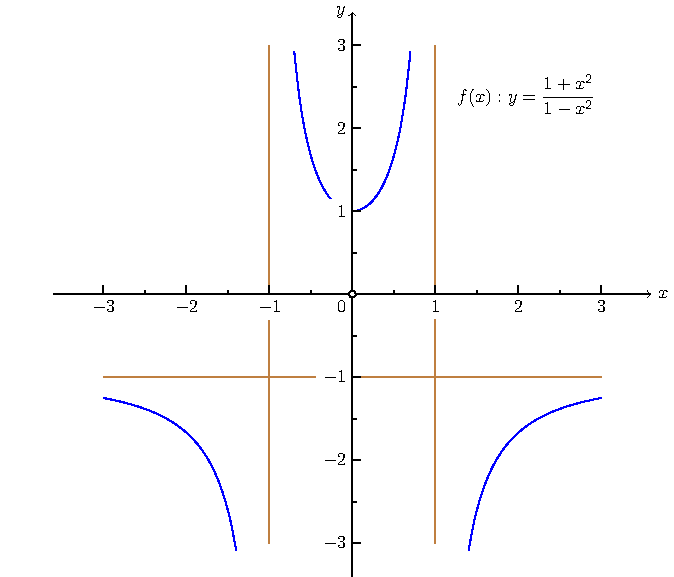
\includegraphics[width=1\linewidth]{MAI007.pdf}
    \captionof{figure}{Graf funkce $f(x):y=\dfrac{1+x^2}{1-x^2}$}
    \label{MAI:fig_007}
  \par}
\end{example}
    %-------------------------------------------------------------------

} %tikzset
%---------------------------------------------------------------------------------------------------
\printbibliography[heading=subbibliography]
\addcontentsline{toc}{section}{Seznam literatury}                 
%--------------------Primitive Functions -----------------------------------------------------------
    %==================================== Primitivní funkce ======================================================
\chapter{Primitivní funkce}
\minitoc
\newpage
  %----------------------------Neurčitý integrál----------------------------------------------------
  \section{Motivace}
    Problém \emph{neurčitého integrálu}, neboli \textbf{primitivní funkce}, lze vyložit velmi jednoduše: 
    Máme podezření, že zadaná funkce \(f(x)\) vznikla derivováním jisté, zatím neznámé, funkce \(F(x)\). 
    Dokážeme ji najít? 
  
    K danému problému můžeme přistupovat také fyzikálně: Zavedením pojmu derivace funkce jsme motivovali 
    důležitým požadavkem definovat okamžitou rychlost pohybu bodu po přímce. Existuje přirozeně i požadavek 
    opačný, tj. nalézt zákon dráhy pohybu bodu po přímce, je-li dána jeho okamžitá rychlost jako funkce 
    času \cite[s.~253]{Brabec1989}. Vše si ukážeme na následujícím příkladu:  
   
    \begin{example}
      Je dána okamžitá rychlost $v$ pohybu bodu po přímce (ose) $x$ rovnicí $v(t) = 2t + 1$, $t\in\langle 
      -\infty,+\infty \rangle$. Najděte zákon dráhy pohybu, je-li známo, že v čase $t = 0$ měl bod polohu 
      $x = x_0$.
      \newline
      \textbf{řešení:}\newline
      Označíme-li $x(t)$ polohu bodu v okamžiku $t$, pak $v(t) = \frac{dx}{dt}$. Hledáme tedy funkci $x = 
      x(t)$, pro níž platí 
      \begin{align}
        \frac{dx}{dt} &= 2t + 1 \qquad x(0) = x_0.  \nonumber \\ 
        \shortintertext{Je ihned patrné, že první podmínce vyhovuje nekonečně mnoho funkcí}
        x(t)          &= t^2 + t + C,           \label{MA:int_ex_09}    \\ 
        \shortintertext{ kde $C$ je libovolná konstanta. Funkce, která splňuje i druhou podmínku 
          (říkáme ji též počáteční podmínka), najdeme z rovnice \ref{MA:int_ex_09} dosazením dané podmínky 
          $t = 0,\ x = x_0$. Dostaneme $x_0 = C$. Dosazením do \ref{MA:int_ex_09} za $C$ plyne hledaný 
          zákon dráhy}
        x(t)          &= t^2+t+x_0.                 \nonumber 
        \shortintertext{Jednoduchou zkouškou se přesvědčíme, že tato funkce splňuje obě dané podmínky a 
          zároveň vidíme, že hledaná primitivní funkce daných vlastností je jediná.}  \nonumber
      \end{align}
    \end{example}\vspace{-1cm}    
    Každé takové funkci, jejíž derivací je daná funkce, budeme říkat \emph{primitivní funkce} k dané 
    funkci. Na uvedeném příkladě je patrné, že k dané funkci může existovat nekonečně mnoho primitivních 
    funkcí. Množinu všech primitivních funkcí se často nazývá \textbf{neurčitým integrálem}. Po tomto 
    názorném uvedení do problému přejděme k přesné formulaci základních pojmů.
    
    \begin{definition} 
      Funkce $F: J\rightarrow \realset$, kde $J\subset \realset$ je interval, se nazývá primitivní funkce k 
      funkci $f$ na intervalu $J$ právě když, pro všechna $x\in J$ je $F'(x) = f(x)$ (v krajních bodech 
      intervalu $J$, pokud k němu patří, jde o derivace jednostranné).
    \end{definition}
    
    \begin{example} 
      K funkci $\sin x$ je primitivní funkcí na libovolném intervalu $J\subset(-\infty,+\infty)$ funkce 
      $-\cos x$, protože $(-\cos x)' = \sin x$. Ale též funkce $3-\cos x$ je primitivní funkcí k funkci $\sin 
      x$, protože $(3 - \cos x)' = \sin x$ pro všechna $x\in(-\infty, \infty)$.
    \end{example}
    
    Je vidět, že rozdíl dvou primitivních funkcí k téže funkci je konstanta. To není náhoda, jak potvrzuje 
    následující věta:
    
    \begin{lemma}
      \begin{enumerate}[label=\itshape\alph*\upshape)]
        \item Je-li funkce $F$ primitivní funkcí k funkci $f$ na intervalu $J$ a $c$ reálná konstanta, pak i 
              funkce $G = F + c$ je primitivní funkcí k funkci $f$ na intervalu $J$.
        \item Jsou-li funkce $F$ a $G$ primitivní funkce k funkci $f$ na intervalu $J$, pak funkce
              $F-G$ je na intervalu $J$ konstantní.
      \end{enumerate} 
      \begin{proof}
        Tvrzení a) plyne z definice protože $G'(x) = [F(x) + c] = F'(x) = f(x)$ pro všechna $x\in
        J$. Tvrzení b) je důsledkem věty \ref{MA1:lem_diff01}.
      \end{proof}
    \end{lemma}
    Neurčitost vyplývá právě z toho, že primitivní funkce není dána jednoznačně, je určena až na konstantu. 
    Značíme
    \begin{equation*}
      \boxed{F(x) = \int f(x)\dx + C}
    \end{equation*}
        
    Jak ale primitivní funkce hledat? V jednoduchých příkladech poslouží tabulka derivací, již čteme „zprava 
    doleva“. (Je dobré si ji uložit do paměti.) Tabulka však pokryje jen velmi málo případů, pouze 
    elementární funkce. Je tedy třeba najít metody, jak při hledání primitivních funkcí postupovat. Nejprve 
    však uvedeme dvě základní pravidla pro primitivní funkce, která plynou z pravidel pro derivování:
    \begin{align}
      \int[f(x)\pm g(x)]\dx &= \int[f(x)\pm g(x)]\dx + \int[f(x)\pm g(x)]\dx \label{MA1:eq_int10} \\
      \int cf(x)\dx         &= c \int f(x)\dx, \qquad \text{\(c\) je konstanta.} \label{MA1:eq_int11}
    \end{align}
  
  \section{Tabulka neurčitých integrálů}\label{MA:chap_tabINT}
    Pokud není nic uvedeno, platí vzorce pro všechna \(x\) a pro všechny hodnoty uvedených
    konstant. Místo platí pro \(x\) z intervalu \((-\infty,0),(0,+\infty)\) píšeme stručně
    \(x\neq0\) apod. Literatura: \cite[p.~396]{Rektorys1963}.
  
    \begin{flalign}
      & \int 0\dx = c                                        &         \label{MA:baseInt01}     \\
      & \int a\dx = ax+c                                     &         \label{MA:baseInt02}     \\
      & \int x^n\dx = \frac{x^{n+1}}{n+1}+c, \qquad
        \begin{cases}
          \forall x\in\realset\,                 
            \text{pro}&\,n\in\naturalset, n>0,         \\
          \forall x\in\realset-\{0\},            
            \text{pro}&\,n\in\naturalset, n<-1,        \\
          \forall x>0,\text{pro}\,n\in\realset\, 
            \text{pro}&\,n\notin\naturalset
        \end{cases}                                          &         \label{MA:baseInt03}     \\
      & \int\frac{1}{x}\dx = 
            \ln\abs{x}+c \hspace{1ex}\forall x\neq0          &         \label{MA:baseInt04}     \\
      & \int e^x \dx       = e^x+c                           &         \label{MA:baseInt05}     \\
      & \int\ln x\dx       = 
          x\ln x - x + c \hspace{1ex}\forall x>0             &         \label{MA:baseInt06}     \\
      & \int a^x \dx     =
          \frac{a^x}{\ln a}+c 
          \hspace{1ex}\forall a>0,\,a\neq1                   &         \label{MA:baseInt07}     \\
      & \int \sin x \dx  = -\cos x                           &         \label{MA:baseInt08}     \\
      & \int \cos x \dx  =  \sin x                           &         \label{MA:baseInt09}     \\
      & \int\frac{1}{\cos^2x}\dx      = 
          \tg x+c   \forall x\neq(2k+1)\pi,\,k\in\naturalset &         \label{MA:baseInt10}     \\ 
      & \int \frac{1}{\sin^2x}\dx     = 
         -\cotg x+c \forall x\neq k\pi,\,k\in\naturalset     &         \label{MA:baseInt11}     \\
      & \int\frac{1}{\sqrt{1-x^2}}\dx =  \arcsin x + c  =  -\arccos x + c 
          \hspace{1ex}\forall x\in(-1,1)\,x\in\realset       &         \label{MA:baseInt12}     \\
      & \int\cosh\dx = \sinh x + c                           &         \label{MA:baseInt13}     \\
      & \int\sinh\dx = \cosh x + c                           &         \label{MA:baseInt14}     \\
      & \int\frac{1}{1+x^2}\dx = \arctg x + c                &         \label{MA:baseInt15}     \\
      & \int \frac{1}{\sqrt{x^2 + 1}}\dx 
        = \ln(x + \sqrt{x^2+1}) + c  
        = \sinh^{-1}x + c                                    &         \label{MA:baseInt16}     \\ 
      & \int \frac{1}{\sqrt{x^2 - 1}}\dx 
        = \ln(x + \sqrt{x^2-1}) + c                   
        = \cosh^{-1}x + c \hspace{1ex}x\in(1,+\infty)        &         \label{MA:baseInt17}     \\
      & \int\frac{1}{\sqrt{x^2+a^2}}\dx 
        = \sinh^{-1} \frac{x}{a} = \ln (x+\sqrt{x^2+a^2})    &         \label{MA:baseInt18}     \\
      & \int \frac{1}{\sqrt{x^2-a^2}}\dx 
        = \cosh^{-1} \frac{x}{a} = \ln (x+\sqrt{x^2-a^2})    &         \label{MA:baseInt19}     
    \end{flalign}
    \vspace{-2.9em}
    \begin{flalign}
      & \int\frac{1}{\sqrt{x^2-1}}\dx 
        = \left\{ 
          \begin{array}{l l}
            \ln\abs{x+\sqrt{x^2-1}}+c      & \quad \text{pro \(\abs{x}>1\)}  \\
            \cosh^{-1}x+c                  & \quad \text{pro \(\abs{x}<1\)}
          \end{array} 
          \right.                                            &         \label{MA:baseInt20}     
    \end{flalign}
    \vspace{-2.9em}
    \begin{flalign}
      & \int\tan x \dx = \ln |\sec x| + c                    &         \label{MA:baseInt21}     
    \end{flalign}
    \vspace{-2.9em}
    \begin{flalign} 
      & \int\sec x \dx = \ln |\sec x + \tan x| + c           &         \label{MA:baseInt22}     
    \end{flalign}
    \vspace{-2.9em}
    \begin{flalign}
      & \int\sec^2 x \dx     = \tan x + c                    &         \label{MA:baseInt23}     
    \end{flalign}
    \vspace{-2.9em}
    \begin{flalign}
      & \int\sec x\tan x \dx = \sec x + c                    &         \label{MA:baseInt24}     \\
      & \int\frac{a}{a^2+x^2}\dx = \tan^{-1}\frac{x}{a}      &         \label{MA:baseInt25}     \\
      & \int\frac{a}{a^2-x^2}\dx = 
          \frac{1}{2}\ln\left|\frac{x+a}{x-a}\right|         &         \label{MA:baseInt26}     \\
      & \int\frac{1}{\sqrt{a^2-x^2}} \dx = 
          \sin^{-1} \frac{x}{a}                              &         \label{MA:baseInt27}     \\
      & \int\frac{a}{x\sqrt{x^2-a^2}}\dx = 
          \sec^{-1} \frac{x}{a}                              &         \label{MA:baseInt28}    
    \end{flalign}     
    
  \section{Metody určení primitivní funkce}
    Procesu hledání primitivní funkce se často říká integrování nebo integrace (od slova “integrál”), což z 
    matematického hlediska znamená provést inverzní operaci k operaci derivování. Smutnou zprávou je, že na 
    rozdíl od derivování neexistuje obecný vzorec pro integrování součinu či podílu, ani obecný vzorec pro 
    integrování složených funkcí. Při hledání integrálů složitějších funkcí se využívá např. 
    \emph{linearita, metoda per partes, substituční metoda}, popř. některé další speciální metody. Řešitel 
    v mnoha případech musí projevit důvtip a intuici, která mu pomůže nalézt primitivní funkci k dané 
    funkci.
  
    % --------------------------Integrace po částech - per partes-------------------------------------------
    \subsection{Integrace po částech - per partes}
      Metoda integrace \emph{per partes} neboli \emph{po částech} využívá vzorce pro derivaci součinu 
      funkcí. Připomeňme si jej: Pro derivaci součinu dvou funkcí \(u(x)\) a \(u(x)\) platí
      \cite[p.~137]{Musilova2009MA1}.
      \begin{align}
        [u(x)v(x)]' &= u(x)'v(x) + u(x)v'(x).  \label{MA:eq_Int29} \\
        \shortintertext{Primitivní funkcí levé strany je \(F(x) = u(x)v(x)\), a tedy}
        u(x)v(x)    &=  \int u'(x)v(x)\dx + \int u(x)v'(x)\dx \nonumber
      \end{align}  
      za předpokladu, že existují obě primitivní funkce na pravé straně. K čemu může tento samozřejmý 
      vzorec sloužit při hledání primitivní funkce? Dejme tomu, že zadaná funkce \(f(x)\), k níž máme 
      hledat funkci primitivní, je tvaru \(f(x) = u'(x)v(x)\), a my si s ní nevíme rady. Je však možné, že 
      bychom si docela dobře poradili s primitivní funkcí k funkci \(g(x) = u(x)v(x)\). A předchozí vzorec 
      umožňuje nahradit výpočet neurčitého integrálu z funkce \(f(x)\) výpočtem neurčitého integrálu z 
      funkce \(g(x)\), tedy
      \begin{equation}\label{ma:eq_perpartes}
        \int u'(x)v(x)\dx = u(x)v(x) - \int u(x)v'(x)\dx 
      \end{equation}
      \begin{example}
        Máme za úkol najít primitivní funkci k funkci \(f(x) = x\sin x\). Představíme-li si ji jako součin 
        \(f(x) = u'(x)v(x)\), kde \(u'(x) = \sin x\), tj. \(u(x) = —\cos x\), a \(v(x)= x\), tj. \(v'(x) 
        = 1\), dostaneme
        \begin{equation*}
          \int x\sin x\dx = -x\cos x + \int\cos x\dx = -x\cos x + \sin x + C.
        \end{equation*}          
      \end{example}
      Není vždy jednoduché rozpoznat, jak máme rozložit funkci \(f(x)\) na součin funkcí \(u'(x)\) a 
      \(v(x)\). Takový rozklad není určen jednoznačně a požadavek na něj bychom mohli (dosti nepřesně) 
      formulovat tak, aby funkce \(v'(x)\) byla jednodušší než v \(v(x)\) (například derivováním polynomu 
      se snižuje jeho stupeň) a funkce \(u'(x)\) a \(u(x)\) aby byly zhruba „stejně složité“ (například 
      \(u'(x) =e^x\), \(u(x) = e^x\), nebo \(u'(x) = \cos x\), \(u(x) = \sin x\), apod.). Spolehlivě 
      používat metodu per partes se však můžeme naučit pouze studiem vyřešených příkladů z literatury a 
      praktickým procvičováním \cite[p.~138]{Musilova2009MA1}.
      
      \begin{example}
        (\emph{Umělý rozklad na součin}): Někdy zadaná funkce \(f(x)\) jako součin vůbec nevypadá, a přesto 
        je použití metody per partes vhodné. Například pro elementární funkci \(f(x) = \ln x\) sice najdeme 
        primitivní funkci \ref{MA:baseInt06} v tabulce základních neurčitých integrálů z odstavce 
        \ref{MA:chap_tabINT}, ale je možné postupovat i jinak. Představme si \(f(x)\) jako součin 
        \(f(x) = 1\cdot\ln x\) a zvolme \[u'(x) = 1 ⇒ u(x) = x, \qquad v(x) = lnx ⇒ v'(x) = \frac{1}{x}\] 
        Pak \[\int \ln\dx = x\ln x - \int x\cdot\frac{1}{x}\dx = x\ln x - x.\]
      \end{example}
  
    %--------------------------- Substituční metoda ----------------------------------------------
    \subsection{Substituční metoda I}
      Tato metoda \emph{substituce} neboli \emph{náhrady} spočívá v tom, že vhodně zvolenou funkci 
      obsaženou v předpisu \(f(x)\) označíme jako novou jednoduchou proměnnou. Čeho tím dosáhneme? 
      Předpokládejme například, že \[f(x)=\varphi'(x)g[\varphi(x)]\] a označme jako novou proměnnou \(u = 
      f(x)\). Že to vypadá, jako bychom se chystali použít vzorec pro derivaci složené funkce? Správně! 
      Dejme tomu, že známe primitivní funkci \(G(u)\) k funkci \(g(u)\). Pak platí
      \begin{align*}
       \left[G\left(\varphi(x)\right)\right]' 
          &= G'\left[\varphi(x)\right]\cdot\varphi'(x) =
             g\left[\varphi(x)\right]\cdot\varphi'(x), \qquad\text{a tedy}   \\
       \int \varphi'(x) g\left[\varphi(x)\right]\dx &=  G\left[\varphi(x)\right]. 
      \end{align*}      
      Na základě těchto úvah formulujeme následující větu:
      \begin{lemma}
        Jestliže
        \begin{equation}\label{ma:eq_subst1}
          \int{f(u)du}=F(u)+C
        \end{equation}
        a $u=\varphi(x)$, pak
        \begin{equation}\label{ma:eq_subst2}
            \int{f[\varphi(x)]\varphi'(x)du}=F(\varphi(x))+C
        \end{equation}
      \end{lemma}
  
      Základem úspěchu při aplikací věty je správný výběr funkce $\varphi(x)$. Praxe je totiž
      taková, že výpočet konkrétních příkladů je schématicky veden od rov. \ref{ma:eq_subst2} ke
      vzorci rov. \ref{ma:eq_subst1}.
      
      \begin{example} Jak poznat kandidáta na substituční metodu I
        Počítejme neurčitý integrál \[\int \frac{x}{\sqrt{x^2+1}}.\]
        Vidíme, že čitatel funkce za integrálem je až na násobení konstantou derivací výrazu pod odmocninou. 
        Při označení \(u=\varphi(x) = x^2 + 1\) dostáváme \(\varphi'(x) = x\), 
        \begin{equation*}
          \int\frac{x}{\sqrt{x^2+1}}\dx = \frac{1}{2}\int\frac{2x}{\sqrt{x^2+1}}\dx
                                        = \frac{1}{2}\int\frac{1}{\sqrt{u}}\dd{u} = \sqrt{u} + C 
                                        = \sqrt{x^2 + 1} + C  
        \end{equation*}
      \end{example}
      
      \begin{example}\label{ma:ex_sub_metoda}$\displaystyle\int{e^{x^{x^2}}dx}$
        \begin{equation*}
            \int{e^{x^{x^2}}dx}=
               \left[
                 \begin{array}{c}u=x^2 \\ du=2xdx\end{array}
               \right]=
               \frac{1}{2}\int{e^udu}=\frac{1}{2}e^u=\frac{1}{2}e^{x^2}+C.
        \end{equation*}
      \end{example}
      \begin{example}$\displaystyle\int{x^3e^{x^4}}dx \qquad x\in R$
        \begin{align*}
          \displaystyle\int{x^3e^{x^4}}dx
             &= 
             \left[
               \begin{array}{cc}
                  u=x^4   & du=4x^3dx \Rightarrow \displaystyle\frac{du}{4} = x^3dx  \\
               \end{array}
             \right]                                                                           \\
             &= \frac{1}{4}\int{e^u}du = \frac{e^u}{4} = \frac{e^{x^4}}{4} + C 
        \end{align*}
      \end{example}

    % -------------------Substituční metoda II----------------------------------------------------------------
    \subsection{Substituční metoda II}
      Druhý typ substituční metody spočívá naopak v tom, že na místo původní proměnné \(x\) dosadíme vhodnou 
      funkci \(x = \psi(t)\). Místo primitivní funkce k funkci \(f(x)\) pak hledáme primitivní funkci k 
      funkci \(g(t) = f[\psi(t)]\psi'(t)\). Skutečně, je-li \(F(x)\) primitivní funkcí k \(f(x)\), pak 
      derivací složené funkce \(G(t) = F[\psi(t)]\) dostaneme
      \begin{equation*}
       G'(t) = F'[\psi(t)]\psi'(t) = f[\psi(t)]\psi'(t) = g(t).
      \end{equation*}
      \begin{example} Náhrada proměnně \(x\) funkcí
        Typické jsou neurčité integrály, které vedou na goniometrické substituce, například
        \[\int\sqrt{1-x^2}\dx\]
        
        Označme \(x=\psi(t)=\sin(t)  \Rightarrow \psi'(t)=\cos(t)\) a můžeme psát
        \begin{align*}
          \int\sqrt{1-x^2}\dx 
            &= \int\sqrt{1-\sin^2t}\cos t\dd{t} = \int\cos^2 t \dd{t} = \int\frac{1+\cos2t}{2}\dd{t}\\
          \frac{1}{2}t+\frac{\sin2t}{4}+C
            &= \frac{1}{2}\arcsin x + \frac{2\sin t\cos t}{4} 
             = \frac{1}{2}\arcsin x + \frac{x\sqrt{1-x^2}}{2} + C.
        \end{align*}
        Správně bychom měli místo \(\sqrt{1 - \sin^2x}\) psát \(\abs{\cos x}\). Vzhledem k tomu, že jde o 
        neurčitý integrál, je možné hledat primitivní funkci na intervalu, kde platí \(\cos x = \abs{\cos 
        x}\).
      \end{example}
      Jistě nám neuniklo, že princip substitučních metod I a II je stejný. Jsou totiž obě založeny na použití 
      pravidla pro derivaci složené funkce.
  
    % ---------Integrování součtu, úprava integrandu a integrování rozkladem----------------------------------
    \subsection{Integrování součtu, úprava integrandu a integrování rozkladem}
      \begin{example}
        Zdroj \cite[s.~29]{Knichal}.
        \begin{equation}\label{MA:int_ex_01}
          \int{\frac{x^4+3x^3-3x^2+3x}{x^2+1}\dx}
        \end{equation}
        Dělením čitatele integrandu jmenovatelem  dostaneme rozklad integrandu na součet funkcí,
        jejich integrály najdeme snadno:
         \begin{equation*} 
           \polylongdiv[style=C,div=:]{x^4+3x^3-3x^2+3x}{x^2+1}
         \end{equation*}
         \begin{align*}
           \shortintertext{Tedy}
           \frac{x^4+3x^3-3x^2+3x}{x^2+1}                 &= x^2+3x-4+\frac{4}{x^2+1} \\
           \intertext{Pro uvedený integrál dostaneme} 
           \int{\frac{x^4+3x^3-3x^2+3x}{x^2+1}\dx}        &=                 \\
           \int{\left(x^2+3x-4+\frac{4}{x^2+1}\right)\dx} &= 
             \frac{x^3}{3}+\frac{3x^2}{2}-4x+4\arctan x + C.
         \end{align*}
      \end{example}
      
      \begin{example}
        Zdroj \cite[s.~29]{Knichal}.
        \begin{equation}\label{MA:int_ex_03}
          \int\frac{3}{(1+x^2)x^2}\dx
        \end{equation}
        Integrand upravíme přičtením a odečtením výrazu $3x^2$ v čitateli zlomku takto:
        \begin{align*}
          \frac{3}{(1+x^2)x^2} 
            &= \frac{3+3x^2-3x^2}{(1+x^2)x^2} = \frac{3}{x^2}-\frac{3}{1+x^2}                      \\  
          \intertext{Tedy v každém otevřeném intervalu, který neobsahuje bod \(x=0\), platí}
          \int{\frac{3}{(1+x^2)x^2}\dx} 
            &= 3\int{\frac{1}{x^2}dx} - 3\int{\frac{1}{1+x^2}dx}                                   \\
            &= -\frac{3}{x}-3\arctan x + C. 
        \end{align*}
      \end{example}
      
      \begin{example}
        Zdroj \cite[s.~30]{Knichal}.
        \begin{equation}\label{MA:int_ex_04}
          \int{\sqrt{1+\cos2x}\dx}
        \end{equation}
        Funkci $\sqrt{1+\cos2x}$ upravíme na základě goniometrické identity \ref{MA1:eq_cos2x}
        \begin{align*}
          1+\cos2x       &= 1+\cos^2x-\sin^2x=2\cos^2x                                         \\
          \shortintertext{takto}
          \sqrt{1+\cos2x}&=\sqrt{2\cos^2x} = \sqrt{2}|\cos x| = \varepsilon\sqrt{2}\cos x,     \\
          \shortintertext{kde}
          \varepsilon &=
            \begin{cases} 
             +1, &  x\in \left(-\frac{\pi}{2}+2n\pi,\frac{\pi}{2}+2n\pi\right), \\
             -1, &  x\in \left(\frac{\pi}{2}+2n\pi,\frac{3\pi}{2}+2n\pi\right),
            \end{cases}                                                                        \\
          \intertext{$n$ je přirozené číslo. Proto pro $x$ ležící v uvedených intervalech je}
          \int\sqrt{1+\cos2x}\dx & = \varepsilon\sqrt{2}\int\cos x\dx 
                                   = \varepsilon\sqrt{2}\sin x + C.
        \end{align*}
      \end{example}
      
      \begin{example}
        Zdroj \cite[s.~30]{Knichal}.
        \begin{equation}\label{MA:int_ex_05}
          \int\cos^2\frac{x}{2}\dx
        \end{equation}
        Integrand upravíme na součet dvou tabulkových integrálů použitím vzorce
        \begin{align*}
          \cos^2\frac{x}{2} &= \frac{1}{2}(1+\cos x)     \\ 
          \shortintertext{takže}
          \int{\cos^2\frac{x}{2}}\dx 
                            &= \frac{1}{2}\int{(1+\cos x)}\dx = \frac{1}{2}(x+\sin x) + C.
        \end{align*}          
      \end{example}
      
      \begin{example}
        Zdroj \cite[s.~30]{Knichal}.
        \begin{equation}\label{MA:int_ex_06}
          \int{\tan^2x}\dx
        \end{equation}
        funkci napíšeme ve tvaru 
        \begin{align*}
          \tan^2x &= \frac{\sin^2x}{\cos^2x}=\frac{1-\cos^2x}{\cos^2x} = \frac{1}{\cos^2x}-1   \\
          \shortintertext{takže}
          \int{\tan^2x}dx &= \int{\left(\frac{1}{\cos^2x}-1\right)}\dx = \tan x - x + C.  
          \intertext{$\forall x\in\left(-\frac{\pi}{2}+k\pi, \frac{\pi}{2}+k\pi\right)$,
                     $k\in\naturalset$.}
        \end{align*}          
        
      \end{example}
      
      \begin{example}
        \begin{equation}\label{MA:int_ex_07} 
          \int\frac{\cos2x}{\cos^2x\cdot\sin^2x}\dx, 
            \qquad (\sin^2x\cos^2x\neq0; x\neq k\frac{\pi}{2}; k\in Z)
        \end{equation} 
       Integrand upravíme pomocí vzorce pro dvojnásobný úhel \ref{MA1:eq_cosx2}:
        \begin{equation*}
          \int\frac{\cos^2x-\sin^2x}{\cos^2x\cdot\sin^2x}\dx = 
            \int\frac{1}{\sin^2x}\dx - \int\frac{1}{\cos^2x}\dx = -\cot x - \tan x + C.
        \end{equation*}
      \end{example}
      
      \begin{example}
       \begin{equation}\label{MA:int_ex_08}
         \int\frac{1}{\cos x\cdot\sin x}\dx, 
           \qquad (\sin x\cos x\neq0; x\neq k\frac{\pi}{2}; k\in Z)
       \end{equation}
       Integrand rozšíříme o funkci $\displaystyle{\frac{1}{\cos^2x}}$
        \begin{equation*}
          \bigintss\dfrac{\dfrac{1}{\cos^2x}}{\dfrac{\sin x\cdot\cos x}{\cos^2x}} \dx = 
          \bigintss\dfrac{\dfrac{1}{\cos^2x}}{\tan x}\dx = \ln\abs{\tan x} + C.
        \end{equation*}            
      \end{example}
  
    %--------------------------- Integrace racionální funkce--------------------------------------
    \subsection{Integrace racionální funkce}
      Některé příklady v předchozím odstavci, (viz např. \ref{MA:int_ex_01} a 
      \ref{MA:int_ex_02}) jsme dělením čitatele integrandu jmenovatelem dostali rozklad
      integrandu na součet racionální funkce (polynomu) a ryze lomené racionální funkce.
      Integrování polynomu je snadné, neboť jde o součet integrálů tvaru $\int c_kx^k dx$, kde
      $k$ je celé nezáporné číslo. Omezíme se tedy na integrování \emph{ryze lomené racionální
      funkce},  tj. funkce ve tvaru $P(x)/Q(x)$, kde $P(x), Q(x)$ jsou polynomy, přičemž stupeň
      polynomu $P(x)$ je menší než stupeň polynomu $Q(x)$. Taková funkce může vzniknout součtem
      několika jednoduchých zlomků.
      
      \begin{example}
        Upravte
        \begin{align*}
          \frac{1}{x-1}+\frac{x+2}{x^2+x+3} 
            & = \frac{x^2+x+3+x^2+x-2}{(x-1)(x^2+x+3)}              \\
            & = \frac{2x^2+2x+1}{x^3+2x-3}
        \end{align*}          
      \end{example}
      
      Jsme tedy vedeni myšlenkou, zda naopak každá ryze lomená racionální funkce se dá rozložit
      na součet jednoduchých zlomků určitého tvaru - budeme jim říkat \texttt{parciální zlomky},
      které umíme integrovat. Tím se budume zabývat v dalších odstavcích. 
            
      \begin{example}
        \begin{equation}
          \int\frac{1}{x^2 - x + 1}\dx, \qquad x\in R
        \end{equation}
        Kvadratický polynom ve jmenovateli upravíme na čtverec $f(x) = (x + m)^2 + n$:
        \begin{align*}
          \int\dfrac{1}{\left(x-\dfrac{1}{2}\right)^2+\dfrac{3}{4}}\dx   &=
            \dfrac{1}{\sqrt{1-\left(\dfrac{1}{2}\right)^2}}\arctan
            \dfrac{x-\dfrac{1}{2}}{\sqrt{1-\left(\dfrac{1}{2}\right)^2}}                       \\
          \dfrac{2}{\sqrt{3}}\arctan\dfrac{2x-1}{\sqrt{3}}               &=
            \dfrac{2\sqrt{3}}{3}\arctan\dfrac{\sqrt{3}(2x-1)}{3} + C
        \end{align*}
      \end{example}     
      
      \begin{definition} Parciální (částečným) zlomkem, budeme nazývat zlomek tvaru
         \begin{equation}
            \frac{A}{(x-\alpha)^k} \qquad\text{nebo}\qquad\frac{Mx + N}{x^2 + px +q}
         \end{equation}  
         $A,\ M,\ N,\ \alpha\ , p,\ q$ reálné $p^2-4q < 0$, $k$ celé nezáporné.         
      \end{definition}
      
      Integrál prvního zlomku, tj. $\displaystyle{\int\frac{A}{(x-\alpha)^k}\dx}$, vypočteme substitucí 
      $x-\alpha=t$, odtud plyne $dx = dt$,
      \begin{equation}\label{MA:int_ex_14}
        \int\frac{A}{(x-\alpha)^k}dx = \int\frac{A}{t^k}dt.
      \end{equation}
      Tento integrál se rovná
      \begin{equation}\label{MA:int_ex_16}
        -\frac{A}{k-1}\frac{1}{(x-\alpha)^{k-1}} + C.
      \end{equation}        
      je-li $k>1$, a rovná se $A\ln|x-\alpha| + C$, je-li $k = 1$. Výsledek platí na každém
      intervalu neobsahujícím bod $\alpha$.
      
       U integrál druhého zlomku uvedeme postup výpočtu pro $k = 1$. 
      \begin{align*}
         \intertext{\(\displaystyle\int{\frac{Mx + N}{x^2+px+q}dx}\)}
           \qquad &=  \int{\frac{Mx}{x^2+px+q}dx} + \int{\frac{N}{x^2+px+q}dx}                     \\  
           \qquad &=  \frac{M}{2}\int{\frac{(2x + p) - p}{x^2+px+q}dx} + 
                     N\int{\frac{1}{x^2+px+q}dx}                                                   \\ 
           \qquad &=  \frac{M}{2}\int{\frac{2x + p}{x^2+px+q}dx} + 
                      \left(N-\frac{Mp}{2}\right)\int{\frac{1}{x^2+px+q}dx.}                   
      \end{align*}  
      
      Z naznačeného postupu je vidět hlavní myšlenka: upravit integrál na lineární kombinaci dvou integrálů, 
      z nichž první má v čitateli integrandu derivaci jmenovatele a je podle příkladu *** roven 
      $\ln|x^2+px+q|$ kde $x^2+px+q >0$ pro $x\in R$ a integrand druhého integrálu má čitatel konstantní.
      
      Výpočet druhého integrálu probíhá takto: 
      \begin{equation}\label{MA:int_ex_10}
        \int\dfrac{1}{x^2+px+q}\dx = 
          \int\dfrac{1}{\left(x+\dfrac{p}{2}\right)^2 + q - \dfrac{p^2}{4}}\dx;
      \end{equation}
      substitucí $x+\dfrac{p}{2} = t\sqrt{q - \dfrac{p^2}{4}}$ dostáváme dále
      \begin{equation*}\label{MA:int_ex_11}
        \bigints{\frac{1}{\displaystyle{\left(x+\frac{p}{2}\right)^2 + q - \frac{p^2}{4}}}}dx 
          =\displaystyle{
            \bigints{
              \frac{\sqrt{q-\frac{p^2}{4}}}{\left(q-\frac{p^2}{4}\right)(t^2+1)}}dt
            }   
      \end{equation*}
      po úpravě dostaneme tabulkový integrál
      \begin{equation}\label{MA:int_ex_12}
        \frac{1}{\sqrt{q-\frac{p^2}{4}}}\int{\frac{dt}{t^2+1}},
      \end{equation}
      jehož řešení je  
      \begin{equation*}\label{MA:int_ex_13}
        \frac{1}{\sqrt{q-\frac{p^2}{4}}}\arctan{t} 
          = \sqrt{q-\frac{p^2}{4}}\arctan\frac{x+\frac{p}{2}}{\sqrt{q-\frac{p^2}{4}}}.     
      \end{equation*}   
      Z postupu je opět vidět hlavní myšlenka: úprava integrandu na tvar $\dfrac{1}{t^2+1}$.
      Jmenovatel $x^2+px+q$ jsme doplnili na úplný čtverec a užili uvedenou substituci (uvažme,
      že $q-\dfrac{p^2}{4}>0$, protože diskriminant $\dfrac{p^2}{4}-q$ trojčlenu $x^2+px+q$ je
      podle předpokladu záporný). Výsledek platí u obou integrálu v intervalu \((-\infty,
      +\infty)\).
      
      % -----------------------Funkce typu {f(x)=\sqrt{ax+b}} ------------------------------------
      \subsubsection*{Funkce typu $\boxed{f(x)=\sqrt{ax+b}}$ :}
         Funkci, jež je dána rovnicí, jež obsahuje polynomy proměnné x  ve výrazu $\sqrt{ax+b}$,
         v němž $ax+b>0$, $a>0$, integrujeme pomocí substituce:
         \begin{equation}\label{ma:eq_sub_fce1}
             u=\sqrt{ax+b},\quad du=\frac{1}{2}\frac{a}{u}dx,\quad dx=2\frac{u}{a}du
         \end{equation}
         Je-li potřeba dosadit do integrované funkce také za $x$, vyjádříme ze substituční
         rovnice $x=\frac{u^2-b}{a}$.
      % ----------------------Funkce typuf(x)=\frac{1}{\sqrt{x^2+a}}, a\neq0 -------------------- 
      \subsubsection*{Funkce typu $\boxed{f(x)=\frac{1}{\sqrt{x^2+a}}}, a\neq0$ :}
         \begin{example}\label{ma:ex_sub_metoda1}$\displaystyle\int{\frac{1}{\sqrt{x^2+a}}dx}$:\vskip0.5mm
           \textbf{Řešení}: Užijeme \textbf{Eulerovu substituci}\vskip1mm 
                            \hskip17mm$u=x+\sqrt{x^2+a},\quad \displaystyle{du=\frac{u}{\sqrt{x^2+a}}dx}$,
                            $\displaystyle{\frac{du}{u}=\frac{dx}{\sqrt{x^2+a}}}.$
           \begin{equation*}
            \int{\frac{1}{\sqrt{x^2+a}}dx}=\int{\frac{du}{u}}=\ln|u|=\ln|x+\sqrt{x^2+a}|+C
           \end{equation*}
         \end{example}
  
    % --------------------------Integrály goniometrických funkcí----------------------------------     
    \subsubsection{Integrace goniometrických funkcí}
      
    % ---------------- Rozklad ryze lomené funkce v parciální zlomky -----------------------------------------
    \subsubsection{Rozklad ryze lomené funkce v parciální zlomky}
      Nechť je dána racionální funkce $R = \frac{P}{Q}$ s reálnými koeficienty. Můžeme
      předpokládat, že je \emph{ryze lomenná}\footnote{tj. stupeň polynomu $P$ je menší než
      stupeň polynomu $Q$}. Pokud by tomu tak nebylo, dostaneme dělením čitetele jmenovatelem
      zlomku součet polynomu a ryze lomené racionální funkce.
      
      \begin{example}$\displaystyle\int{\frac{8x-31}{x^2-9x+14}}dx$\cite[s.~90]{Knichal}\newline
        Kořeny polynomu ve jmenovateli $\alpha_1 = 2$, $\alpha_2 = 7$ jsou jednoduché - každému z
        nich bude v rozkladu odpovídat jen jeden člen $$\frac{8x-31}{x^2-9x+14} = \frac{A}{x-2}
        + \frac{B}{x-7}.$$ Členy mnohočlenu na pravé straně seřadíme podle mocnin $x$ $$8x-31 =
         x(A+B)+(7A-2B).$$ Porovnáním odpovídajících si koeficientů dostaneme
        \begin{align*}
          8   &=   \; A + \, B \\
          -31 &= -7A - 2B
        \end{align*}
        Řešením této soustavy je $A = 3, B = 5$. Platí tedy (pro všechna $x \neq 2$ a $x \neq 7$)
        $$\frac{8x-31}{x^2-9x+14} = \frac{3}{x-2} + \frac{5}{x-7}.$$
        \begin{align*}
          \int{\frac{8x-31}{x^2-9x+14}}dx 
            &= \int{\frac{3}{x-2}}dx + \int{\frac{5}{x-7}}dx      \\
            &= 3\ln|x-2| + 3\ln|x-7| + C.
        \end{align*}
        Výsledek platí v každém intervalu, který neobsahuje body $x = 2$,$x = 7$.
      \end{example}
      
      \begin{example}\label{MA:eq_ex1}$\displaystyle\int{\frac{19x+15}{x^2-x-2}}dx \qquad x\in
        R-\{1,2\} $ \newline Kořeny polynomu ve jmenovateli $\alpha_1 = -1$, $\alpha_2 = 2$ jsou
        jednoduché - každému z nich bude v rozkladu odpovídat jen jeden člen: 
        \begin{align*}
          \frac{19x+15}{x^2-x-2}     &= \frac{A}{x+1} + \frac{B}{x-2} \\
                           19x +15   &= A(x-2) + B(x+1)               \\
                           19x +15   &= x(A+B) - 2A + B               \\
                           19        &= A + B                         \\
                                15   &=        - 2A + B
        \end{align*}              
        Řešením této soustavy je $A = \frac{4}{3}$, $B = \frac{53}{3}$.
        \begin{equation*}
          = \frac{4}{3}\int{\frac{1}{x+1}}dx+\frac{53}{3}\int{\frac{1}{x-2}}dx 
          = \frac{4}{3}\ln|x+1| - \frac{53}{3}\ln|x-2| +  C
        \end{equation*}      
      \end{example}
  
      \begin{example}
        $\displaystyle\int{\frac{2x^2+34x+14}{x^3-4x^2-x-4}}dx$\cite[s.~90]{Knichal}\newline
        Polynom $Q(x)=x^3-4x^2-x-4$ má kořeny $\alpha_{1,2}=\pm1$, $\alpha_{3}=-4$, které jsou
        jednoduché tj. $Q(x)=(x-1)(x+1)(x+4)$ $$\frac{2x^2+34x+14}{x^3-4x^2-x-4} =
        \frac{A}{x-1}+\frac{B}{x+1}+\frac{C}{x+4}$$ Vynásobíme-li tuto rovnici společným
        jmenovatelem zlomků pravé strany (polynomem $Q(x)$), dostaneme
        \begin{align*}
          2x^2+34x+14 &= A(x+1)(x+4)+B(x-1)(x+4)+C(x-1)(x+1) \\
          \intertext{čili}
          2x^2+34x+14 &= A(x^2+5x+4)+B(x^2+3x-4)+C(x^2-1) \\
          2x^2+34x+14 &= (A+B+C)x^2+(5A+3B)x + (4A-4B-C)
        \end{align*}
        Porovnáním odpovídajících si koeficientů u stejných mocnin $x$  dostaneme pro nez\-ná\-mé
        koeficienty $A, B, C$ soustavu rovnic
        \begin{align*}
        % \nonumber to remove numbering (before each equation)
           A+   B + C &= 2 \\
          5A + 3B     &= 34 \\
          4A - 4B - C &= 14
        \end{align*}
        Řešením této soustavy je $A = 5, B = 3, C = -6$ a tedy
        $$\frac{2x^2+34x+14}{x^3-4x^2-x-4} = \frac{5}{x-1}+\frac{3}{x+1}-\frac{6}{x+4}$$
        \begin{align*}
          \int{\frac{2x^2+34x+14}{x^3-4x^2-x-4}}dx 
            &= \int{\frac{5}{x-1}}dx + \int{\frac{3}{x+1}}dx + \int{\frac{6}{x+4}}dx            \\
            &= 5\ln|x-1| +  3\ln|x+1| - 6\ln|x+4| +C.
        \end{align*}
      \end{example}
  
      \begin{example}$\displaystyle{\int\frac{2x+3}{2x^3+2}dx} \qquad x\in R-{-1}$\newline
        a
      \end{example}

  % ---------------- Sbírka řešených příkladů ----------------------------------------------------------------
  \newpage
  \section{Sbírka řešených příkladů}
    Hledej primitivní funkce \(F(x)\) k následujícím funkcím
    
  \begin{example}\(\displaystyle\int{xe^x\dx}\)
    \begin{equation*}
        \int{xe^xdx}=
          \left[\begin{array}{cc}
            u=x   & dv=e^x \\
            du=dx & v=e^x
          \end{array}\right]=
          xe^x-\int{e^x\dx} = xe^x - e^x+C
    \end{equation*}
  \end{example}
  
  \begin{example}$\displaystyle\int{\arctan xdx} \qquad x\in R$
    \begin{align*}
       \int{\arctan xdx}                      &= 
         \left[\begin{array}{cc} 
                  u =\arctan x                     &  dv= 1  \\ 
                 du =\displaystyle\frac{1}{x^2+1}  &   v= x
               \end{array}
         \right]  =                                                                  \\
       x\arctan x-\int\frac{x}{x^2+1}         &= 
         \left[\begin{array}{c} 
                  x^2 + 1 = t  \Rightarrow 2xdx = dt        \\ 
                      xdx = \displaystyle{\frac{dt}{2}}
               \end{array} 
         \right] =                                                                   \\ 
       x\arctan x-\frac{1}{2}\int\frac{dt}{t} &= x\arctan x-\frac{1}{2}\ln|t|        \\
         &=   x\arctan x-\frac{1}{2}\ln|1+x^2|+C                                     \\
    \end{align*}
  \end{example}
  
  \begin{example}$\displaystyle\int{\sqrt{x^2+a}dx}$, kde $a\neq0, x^2+a>0$
    \begin{align*}
      \int{\sqrt{x^2+a}\dx}                           &=
        \left[
          \begin{array}{cc} 
             u =\sqrt{x^2+a}              & dv = 1 \\ 
            du =\displaystyle
                  \frac{x}{\sqrt{x^2+a}}  &  v = x
          \end{array}
        \right]                                                                                   \\
      x\sqrt{x^2+a}-\int{\frac{x^2}{\sqrt{x^2+a}}\dx} &= 
        \displaystyle{x\sqrt{x^2+a}-\int{\frac{x^2+a-a}{\sqrt{x^2+a}}\dx}}                        \\
      \int{\sqrt{x^2+a}\dx}                           &= 
        \displaystyle{x\sqrt{x^2+a}-\int{\sqrt{x^2+a}\dx} + \int{\frac{a}{\sqrt{x^2+a}}\dx}}      \\
      \int{\sqrt{x^2+a}\dx}                           &= 
        \frac{1}{2}\left[x\sqrt{x^2+a}+a\int{\frac{1}{\sqrt{x^2+a}}}\dx\right]
    \end{align*}
    Integrál na pravé straně vyjádříme podle příkladu \ref{ma:ex_sub_metoda1}
    $\displaystyle{\int{\frac{1}{\sqrt{x^2+a}}\dx}}$ a výsledek do\-sta\-ne\-me ve tvaru
    $$\int\displaystyle{{\sqrt{x^2+a}\dx}=\frac{1}{2}\left[x\sqrt{x^2+a}+a\ln{|x +
    \sqrt{x^2+a}|}\right]}$$
  \end{example}
  
  \begin{example}
    \begin{equation}\label{MA:int_ex_02}
      \int{\frac{2x^4-5x^2+14x+13}{x^2-x-2}\dx} \qquad x\in R - \{1,2\}
    \end{equation}
    Dělením čitatele integrandu jmenovatelem dostaneme rozklad integrandu na součet funkcí, jejich integrály 
    najdeme snadno:
    \begin{widetext}
      \begin{equation*}
        \polylongdiv[style=C,div=:]{2x^4-5x^2+14x+13}{x^2-x-2}
      \end{equation*}
    \end{widetext}
    Zbytek po dělení představuje integrál, jež je počítán v příkladu \ref{MA:eq_ex1} a proto ho vynecháme.
    \begin{align*}
       &= 2\int x^2\dx + 2\int x\dx + \int\dx + \int\frac{19x+15}{x^2-x-2}\dx     \\
       &= \frac{2}{3}x^3 + x^2 + x + \frac{4}{3}\ln|x+1| - \frac{53}{3}\ln|x-2| + C 
    \end{align*}                
  \end{example}
    
  \printbibliography[heading=subbibliography]
  \addcontentsline{toc}{section}{Seznam literatury}
%--------------------an Integrals of functions of one real variable --------------------------------
    %====================================================================================================
% --------------------------------------------- Definite Integral -----------------------------------
\chapter{Určitý integrál}
\minitoc
\newpage  
\section{Motivace} 
  %----------------------------------
  % image: MAI_animated_integral.tex label: \label{MAI:fig_anim_int}
    % \documentclass{book}
% \usepackage{ifthen}
% \usepackage{tikz}
%   \usetikzlibrary{intersections}
%   \usetikzlibrary{calc}
% \usepackage{animate}

\newcounter{r}
\newcommand{\escalar}[1]{
\setcounter{r}{#1 * #1 * #1}
}
%
\newcounter{m}
\setcounter{m}{0}
\newcounter{mc}

% \begin{document}
    %\begin{frame}[fragile]{Animated Integral}
      %\centering
      \protect  % JAFA příkaz protect pomohl -> nemusí být \begin{frame}, který funguje divně (vysází se obsah
                % závorek, tj. [fragile]{Animated Integral})
        \begin{animateinline}[loop, poster = first, controls, palindrome]{2}
          \whiledo{\them < 21}{
            \begin{tikzpicture}[scale=1.25]
              \draw[red,thick,<->] (-1,1) parabola bend (0,0) (2.1,4.41)
                  node[below right] {$y=x^2$};
              \draw[loosely dotted] (-1,0) grid (4,4);
              %\path[use as bounding box] (-2,-1) rectangle (5,5);
              \draw[->] (-0.2,0) -- (4.25,0) node[right] {$x$};
              \draw[->] (0,-0.25) -- (0,4.25) node[above] {$y$};
              \foreach \x/\xtext in {1/1, 2/2, 3/3}
                \draw[shift={(\x,0)}] (0pt,2pt) -- (0pt,-2pt) node[below] {$\xtext$};
              \foreach \y/\ytext in {1/1, 2/2, 3/3, 4/4}
                \draw[shift={(0,\y)}] (2pt,0pt) -- (-2pt,0pt) node[left] {$\ytext$};
              %
              \setcounter{mc}{\value{m}*\value{m}}
              \shade[top color=blue,bottom color=gray!50]
                  (0,0) parabola (0.1*\them,0.01*\themc) |- (0,0);
              \escalar{\them}
              \draw (3cm,2pt) node[above]
                {$\displaystyle\int\limits_0^{\them/10}\!\!x^2\mathrm{d}x=\displaystyle\frac{\ther}{3000}$};
              \draw[fill=orange,color=orange] (0.1*\them,0.01*\themc) circle (0.5pt);
            \end{tikzpicture}
            %
            \stepcounter{m}
            \ifthenelse{\them < 21}{
                    \newframe
            }{
                \end{animateinline}\relax % BREAK
            }
          } % END \whiledo...
      \label{MAI:fig_anim_int}
    %\end{frame} 
  
% \end{document}  
  %---------------------------------- 

\subsection{Výpočet integrálu}
    \begin{example}Metodou per partes spočítejte integrály:$\displaystyle\int_1^{ln5}{(x+1)e^xdx}$
      \begin{align*}
        \int{(x+1)e^xdx} &= \int{e^xdx}+\int{x\cdot e^xdx} \\
                         &= e^x + (x-1)e^x = xe^x \\
        \int_1^{ln5}{(x+1)e^xdx} &= [xe^x]_1^{ln5} = 5ln5-e\\
      \end{align*}
      kde integrál
      \begin{equation*}
          \int{xe^xdx}=
            \left[\begin{array}{cc}
              u=x   & dv=e^x \\
              du=dx & v=e^x
            \end{array}\right]=
            xe^x-\int{e^xdx} = xe^x - e^x+C
      \end{equation*}
    \end{example}

\newpage
\section{Vlastnosti určitého integrálu}
  V této kapitole mluvíme o spojitých funkcích $\Rightarrow$ příslušné integrály tedy vždy
  existují. Čerpáno z knih:
  \cite{Knichal}.

  \begin{lemma}
    \textbf{První věta o střední hodnotě integrálního počtu}: Je-li funkce $f(x)$ spojitá v
    intervalu $\langle a, b\rangle$, existuje alespoň jeden takový bod $c\in(a, b)$, že platí

    \begin{equation}\label{MA:eq_av1}
      \int_a^b f(x)dx = (b-a)f(c).
    \end{equation}
  \end{lemma}

  \begin{proof} Použitím Lagrangeovy věty napsané pro funkci $F(x)$, primitivní na intervalu
    $\langle a, b\rangle$ k dané funkci $f(x)$. Podmínky věty jsou zřejmě splněny: $F(x)$ je
    spojitá na intervalu $\langle a, b\rangle$ a má všude derivaci $F'(x)= f(x)$. Tedy existuje
    alespoň jeden bod $c\in(a, b)$,
    
      %----------------------------------
        % image: MAI_rolle_02.tex label: \label{MA:fig_rolle_02} 
        % \documentclass{article}
% \usepackage{tikz}
% \usetikzlibrary{decorations.markings}
% \usetikzlibrary{intersections}
% \usepackage{wrapfig}                   % Floats, Figures and Captions  
% \usetikzlibrary{calc}

% \begin{document}
 
    \begin{figure}[hb!]
        \centering
        \begin{tikzpicture}
           [scale=3,line cap=round,
            % Styles
              axes/.style=,
              important line/.style={very thick},
              information text/.style={rounded corners,fill=red!10,inner sep=1ex}]
          \begin{scope}[axes]     
            \draw[->] (-0.2, 0) -- (1.5, 0) node[right] {$x$} coordinate(x axis);
            \draw[->] (0, -0.2) -- (0, 1.5) node[left] {$y$} coordinate(y axis);
          \end{scope}
          % my function  
           \draw[very thick,red](1.5,1.4) node[left=1pt,fill=white]{$y=f(x)$};
           \coordinate [label={[blue]left:$D$}] (D) at (0.3,0.5);
           \coordinate [label={[blue]right:$C$}] (C) at (1.2,1.2);
           \draw[name path=func] (D) .. controls (1.0,0.5) and (0.5,1.2) .. (C);
          % horizontal line
           \draw[name path=my_line, gray, dotted] (0.75,0) node[below, red]{$c$} -- (0.75,0.9);
          % intersection between vertical line and my function
           \fill[red, opacity=0.5, name intersections={of=func and my_line, by={intersect}}]
                (intersect) circle (1pt);
          % x-axis labels
           \draw[gray, dotted, text = blue] (D) -- +(0,-0.5) 
              node [label={[xshift=-0.2cm, yshift=0.5mm]$A$},below] (A) {$a$};
           \draw[gray, dotted, text=blue] (C) -- +(0,-1.2)
              node [label={[xshift=0.2cm, yshift=0.5mm]$B$},below] (B) {$b$};
           \draw[red](-0.05,-0.08) node[left=1pt,fill=white]{$0$};
          % y-axis labels
           \draw[gray, dotted] let \p1=(D), \p2=(intersect), \p3=(C) in (\x1,\y2)
              -- +(-\x1,0) node[left, red]{$f(c)$} 
              -- (\x1,\y2) node[above, blue] (F) {$F$} 
              -- (\x3,\y2) node[right, blue]{$E$}; 
          % dotted line between F and D
           \draw[gray, dotted] (F) -- (D);
        \end{tikzpicture}
        \caption{ }\label{MAI:fig_rolle_02}
    \end{figure}
  
%\end{document}  
      %----------------------------------   
    
      že $$F(b)-F(a) = (b-a)F'(c),$$ čímž je věta dokázána, neboť $F(b)-F(a) = \int_a^bf(x)dx$ a
      $F'(c) = f(c)$. Funkční hodnotu $f(c)$, danou podle (\ref{MA:eq_av1}) rovnicí  
      \begin{equation}\label{MA:eq_av2}
         f(c) = \frac{1}{b-a}\int_a^b f(x)dx
      \end{equation}
      nazýváme \texttt{střední hodnotou}.
  \end{proof}

  Pro spojitou nezápornou funkci $f(x)$, lze větu o střední hodnotě jednoduše geometricky
  interpretovat dle (obr.\ref{MAI:fig_rolle_02}). Levá strana (\ref{MA:eq_av1}) určuje obsah
  křivočarého lichoběžníka $ABCD$, pravá strana obsah obdélníka $ABEF$. Podle této věty nabývá
  funkce $f(x)$ aspoň v jednom bodě intervalu $(a, b)$ takové hodnoty $f(c)$, že uvažovaný
  křivočarý lichoběžník má stejný obsah jako obdélník o základně $b-a$ a výšce $f(c)$ (str. 155
  knihy \cite{Knichal}).

  \begin{example} Určete střední hodnotu $i_s$ střídavého proudu $$i(t) = I_0\sin\omega t$$ v
    časovém intervalu $\langle 0, \frac{T}{2}\rangle$ (v průběhu jedné poloviny periody). $I_0$ je
    maximální hodnota proudu (obr. \ref{MA:fig_Iav_exam}), perioda $T$ je dána vztahem $T =
    \frac{2\pi}{\omega}$
    %----------------------------------
      % image: MAI_rolle_02.tex label: \label{MA:fig_Iav_exam}
      % \documentclass{article}
% \usepackage{tikz}
% \usetikzlibrary{decorations.markings}
% \usetikzlibrary{intersections}
% \usetikzlibrary{calc}

% \begin{document}
 
      {\centering
       \begin{tikzpicture}[domain=0:2*pi] 
         \draw[xstep=pi/4, ystep=0.5, dashed, color=gray] (-0.1,-1.6) grid (2*pi,1.6); 
         \draw[->] (-0.2,0) -- (7,0) node[right] {$t$}; 
         \draw[->] (0,-2.5) -- (0,2) node[above] {$i(t)$}; 
         % text 
         \node[below left](0,0){$0$};
         \node[left, color=blue] at (0,1.0) {$I_0$}; 
         % period
         \draw[<->] (0,-2) -- (pi,-2) node[above]{$T$} --(2*pi,-2);
         \draw (2*pi,-2.2) -- (2*pi,0); 
         \foreach \x/\xtext in {0.5*pi/\frac{\pi}{2} ,pi/\pi, 1.5*pi/\frac{3\pi}{2}, 2*pi/2\pi}
         \draw[shift={(\x,0)}] (0pt,2pt) -- (0pt,-2pt) node[below, fill=white] {$\xtext$};  
         \node[below right, color=blue, fill=white] at (2.5,1.0) {$i(t) = I_0\sin\omega t$};
         % function 
         \draw[color=blue, smooth]   plot (\x,{sin(\x r)}); 
       \end{tikzpicture}  
       \captionsetup{type=figure}   
       \captionof{figure}{}\label{MA:fig_Iav_exam}
    \par}
  
%\end{document}  
    %----------------------------------

    Podle \ref{MA:eq_av2} bude
    \begin{align*}
     i_s &=  \frac{2}{T}
             \int_0^{\frac{T}{2}}I_0\sin\omega t\dd{t} =
             \frac{2I_0}{T}\left[-\frac{\cos\omega t}{\omega}\right]_0^{\frac{T}{2}}        \\
         &=  \frac{2I_0}{T}\frac{1}{\omega}\left(-\cos\frac{\omega T}{2}+ \cos 0\right)     \\
         &=  \frac{2I_0}{2\pi}(-\cos\pi + \cos 0) = \frac{2}{\pi}I_0 \doteq 0,637 I_0.
  \end{align*}

  Tato hodnota se rovná intenzitě elektrického proudu, při kterém by vodičem v průběhu uvažované
  poloviny periody prošel stejný elektrický náboj jako při proudu střídavém.
  \end{example}

  \begin{example} Efektivní hodnota $i_{ef}$ střídavého proudu $$i(t) = I_0\sin\omega t$$ (viz
    předchozí příklad) je definována jako odmocnina ze střední hodnoty funkce $i^2(t)$ v průběhu
    jedné periody $T = \frac{2\pi}{\omega}$. Tedy
    \begin{align*}
      i_{ef}^2 &= \frac{1}{T}\int_0^T I_0^2\sin^2\omega t\dd{t} = 
                  \frac{1}{T}\int_0^T \frac{I_0^2}{2}(1- \cos2\omega t)\dd{t}           \\
               &= \frac{I_0^2}{2T}
                  \left[
                    t-\frac{\sin2\omega t}{2\omega}
                  \right]_0^T = \frac{I_0^2}{2}
    \end{align*}
    neboť $\sin2\omega T=\sin4\pi = 0.$ Odtud $$i_{ef} = \frac{I_0}{\sqrt{2}}.$$ Střídavý proud
    $i(t) = I_0\sin\omega t$ má na témže odporu stejný výkon jako stejnosměrný proud o intenzitě
    $i = 0,707I_0$.
  \end{example}
  Následující věta může být využita k odhadu některých integrálů
  \begin{lemma}
    \textbf{Druhá věta o střední hodnotě integrálního počtu}: Jsou-li funkce $f(x)$ a $g(x)$
    spojité v intervalu $\langle a, b \rangle$ a je-li funkce $g(x)$ v $\langle a, b \rangle$
    nezáporná a nerostoucí, existuje alespoň jeden bod $c\in\langle a, b \rangle$ tak, že platí
    \begin{equation}\label{MA_eq_av3}
        \int_a^b f(x)g(x) = g(a)\int_a^c f(x)dx.
    \end{equation}
  \end{lemma}
  Zcela obdobnou větu lze vyslovit pro případ, že $g(x)$ je v intervalu $\langle a, b \rangle$
  nezáporná a neklesající, tj. na pravé straně \ref{MA_eq_av3} je pak integrál $g(b)\int_c^b
  f(x)dx$

  \begin{example} Odhadněte hodnotu integrálu
    \begin{equation}\label{MA_eq_sinx_x}
        \int_{100\pi}^{1000\pi}\frac{\sin x}{x}dx
    \end{equation}
    Řešení: Funkce $f(x) = \sin x$ a $g(x) = \frac{1}{x}$ jsou v uvažovaném intervalu $\langle
    100\pi, 1000\pi \rangle$ spojité a funkce $g(x)$ je kladná a nerostoucí.
    \begin{equation*}
      \int_{100\pi}^{1000\pi}\frac{\sin x}{x}dx = 
      \frac{1}{100\pi}\int_{100\pi}^c\sin xdx =\frac{1}{100\pi}\left(\cos100\pi - \cos c\right)
    \end{equation*}
    kde $c$ je kladné číslo z intervalu $\langle 100\pi, 1000\pi \rangle$. Dále pro všechna
    $c\in\langle 100\pi, 1000\pi \rangle$ platí $0\leq1-\cos c\leq2$, takže
    \begin{equation*}
        0\leq\int_{100\pi}^{1000\pi}\frac{\sin x}{x}dx\leq \frac{1}{50\pi}.
    \end{equation*}
  \end{example}   
%---------------------------------------------------------------------------------------------------
\printbibliography[heading=subbibliography]
\addcontentsline{toc}{section}{Seznam literatury}
%---------------------Řady--------------------------------------------------------------------------
    \input{../src/MAI/chapters/Series.tex}    
%---------------------------------------------------------------------------------------------------  
